\chapter{Weak Convergence} %\seb{$\checkmark$} }
\label{ch:weakconv}

\epigraph{
At the age of twenty-one he wrote a treatise upon the Binomial Theorem, %which has had a European vogue. On the strength of it he won the Mathematical Chair at one of our smaller universities, 
and had, to all appearances, a most brilliant career before him.
}
{\textsc{Sherlock Holmes}} %\\The Final Problem

In this chapter we present a weak convergence result which is identical to Theorem~\ref{thm:FDDconv} except that the mode of convergence is strengthened from convergence of the finite-dimensional distributions to weak convergence. 
Weak convergence is desirable because it implies convergence of a strictly larger class of functions of genealogies, granting access to the distributions of statistics such as the time to the sample MRCA, the total branch length, and the probability that the MRCA of a subsample is equal to the sample MRCA.
%\seb{okay, technically if this one is going to be a ``statistic'', I'm talking about the indicator on this event}. 

The extension from Theorem~\ref{thm:FDDconv} to weak convergence requires an additional tightness argument. The proof is rather long-winded since we do not have the strong assumptions on the dynamics of the interacting particle system that are exploited for example in \textcite{mohle1999}. The proof is broken down into a series of technical results which culminate in Theorem~\ref{thm:weakconv}. The overall structure of the proof is depicted graphically in Figure~\ref{fig:weakconv_structure}.


We start by defining a suitable metric space.
Let $\mathcal{P}_n$ be the space of partitions of $\{1,\dots,n\}$.
Denote by $\mathcal{D}$ the set of all functions mapping $[0,\infty)$ to $\mathcal{P}_n$ that are right-continuous with left limits.
Our rescaled genealogical process $(\mathcal{G}^{(n,N)}_{\tau_N(t)})_{t\geq0}$ and our encoding of the $n$-coalescent are piecewise-constant functions mapping time $t\in[0,\infty)$ to partitions, and thus live in the space $\mathcal{D}$.
Finally, equip the space $\mathcal{P}_n$ with the discrete metric,
\begin{equation*}
\rho(\xi,\eta) 
= 1- \delta_{\xi\eta} 
:= \begin{cases}
    0 &\text{if } \xi=\eta \\
    1 &\text{otherwise}
\end{cases}
\end{equation*}
for any $\xi, \eta \in \mathcal{P}_n$.


\begin{theorem}\label{thm:weakconv}
Let $\nu_t^{(1:N)}$ denote the offspring numbers in an interacting particle system satisfying \ref{standing_assumption} and such that, for any $N$ sufficiently large, for all finite $t$, $\Prob[ \tau_N(t) = \infty ] =0$. Suppose that there exists a deterministic sequence $(b_N)_{N\in\mathbb{N}}$ such that ${\lim}_{N\to\infty} b_N =0$ and%\amj{This bound comparse conditional expectations, so pedantically I suppose we should say that it holds almost surely?}
\begin{equation}\label{eq:mainthmcondition2}
\frac{1}{(N)_3} \sum_{i = 1}^N \Et\left[ (\nu_t^{(i)})_3 \right]  \leq b_N \frac{1}{(N)_2} \sum_{i = 1}^N \Et\left[ (\nu_t^{(i)})_2 \right]
\end{equation}
almost surely for all $N$, uniformly in $t \geq 1$.
Then the rescaled genealogical process $(G_{\tau_N(t)}^{(n,N)})_{t\geq0}$ converges weakly in $(\mathcal{D}, \rho)$
to Kingman's $n$-coalescent as $N \to \infty$.
\end{theorem}

\begin{proof}[Proof of Theorem~\ref{thm:weakconv}]
The structure of the proof follows \textcite{mohle1999}, albeit with considerable technical complication due to the dependence between generations (non-neutrality) in our model.
To make it digestible, the proof is broken down into a number of results which are organised into sections; the relationships between these are shown in Figure~\ref{fig:weakconv_structure}.

Since we already have convergence of the finite-dimensional distributions (Theorem~\ref{thm:FDDconv}), strengthening this to weak convergence requires relative compactness of the sequence of processes $\{ (G_{\tau_N(t)}^{(n,N)})_{t\geq0} \}_{N\in\mathbb{N}}$.

\textcite[Chapter 3, Corollary 7.4]{ethier1986} provide a necessary and sufficient condition for relative compactness: $\mathcal{P}_n$ is finite and therefore complete and separable, and the sample paths of $(G_{\tau_N(t)}^{(n,N)})_{t\geq0}$ live in $\mathcal{D}$, so the conditions of their corollary are satisfied.
The corollary states that the sequence of processes $\{ (G_{\tau_N(t)}^{(n,N)})_{t\geq0} \}_{N\in\mathbb{N}}$ is relatively compact if and only if the following two conditions hold:
\begin{enumerate}
\item \label{item:relcomp1} For every $\epsilon>0$, $t\geq 0$ there exists a compact set $\Gamma \subseteq \mathcal{P}_n$ such that
\begin{equation*}
\liminf_{N\to\infty} \Prob[ G_{\tau_N(t)}^{(n,N)} \in \Gamma ] 
\geq 1-\epsilon
\end{equation*}
\item \label{item:relcomp2} For every $\epsilon>0$, $t>0$ there exists $\delta>0$ such that
\begin{equation*}
\liminf_{N\to\infty} \Prob[ \omega(G_{\tau_N(\cdot)}^{(n,N)}, \delta, t) < \epsilon ] 
\geq 1-\epsilon
\end{equation*}
where $\omega$ is the modified modulus of continuity:
\begin{equation*}
\omega(G_{\tau_N(\cdot)}^{(n,N)}, \delta, t) := \inf \max_{i \in [K]} 
        \sup_{u,v \in [T_{i-1}, T_i)} \rho\left( 
        G_{\tau_N(u)}^{(n,N)}, G_{\tau_N(v)}^{(n,N)} \right)
\end{equation*}
with the infimum taken over all partitions of the form $0=T_0<T_1<\cdots <T_{K-1} <t \leq T_K$ (for any $K$) such that $\min_{i\in[K]} (T_i - T_{i-1}) > \delta$. 
\end{enumerate}
In our case, Condition~\ref{item:relcomp1} is satisfied automatically with $\Gamma = \mathcal{P}_n$, since $\mathcal{P}_n$ is finite and hence compact. 
Intuitively, Condition~\ref{item:relcomp2} ensures that the jumps of the process are well-separated. 
In our case where $\rho$ is the discrete metric, we see that $\rho( G_{\tau_N(u)}^{(n,N)}, G_{\tau_N(v)}^{(n,N)} )$ is equal to 1 if there is a jump between times $u$ and $v$, and 0 otherwise.
Taking the supremum and maximum then indicates whether there is a jump inside any of the intervals of the given partition; this can only be equal to zero if all of the jumps up to time $t$ occur exactly at the times $T_0, \dots, T_K$. 
The infimum over all allowed partitions, then, can only be equal to zero if no two jumps occur less than $\delta$ (unscaled) time apart, because of the restriction we placed on these partitions.

The proof is concentrated on proving Condition~\ref{item:relcomp2}.
To do this, we use a coupling with another process that contains all of the jumps of the genealogical process, with the addition of some extra jumps. This process is constructed in such a way that it can be shown to satisfy Condition 2, and hence so does the genealogical process.

Define $p_t := \max_{\xi\in \mathcal{P}_n} \{1 - p_{\xi\xi}(t)\} = 1 - p_{\Delta\Delta}(t)$, where $\Delta$ denotes the trivial partition of singletons $\{ \{1\},\dots, \{n\} \}$. For a proof that the maximum is attained at $\xi = \Delta$, see Lemma \ref{thm:maximum_pr}. 
Following \textcite{mohle1999}, we now construct the two-dimensional Markov process $(Z_t, S_t)_{t \in \mathbb{N}_0}$ on $\mathbb{N}_0 \times \mathcal{P}_n$ with transition probabilities
\begin{align}
\Prob[ Z_t = j , S_t = \eta \mid Z_{t-1} = i&, S_{t-1} = \xi, \mathcal{F}_\infty] \notag\\
&= \begin{cases}
1 - p_t &\quad \text{if } j=i \text{ and } \xi=\eta \\
p_{\xi\xi}(t) + p_t - 1  &\quad \text{if } j=i+1 \text{ and } \xi=\eta \\
p_{\xi\eta}(t) &\quad \text{if } j=i+1 \text{ and } \xi\neq\eta \\
0 &\quad \text{otherwise} 
\end{cases}
\label{eq:constructed_chain}
\end{align}
and initial state $Z_0=0$, $S_0 = \Delta$.
Unlike the corresponding process in \textcite{mohle1999}, in our case the transition probabilities depend on offspring counts, thus the process is only Markovian conditional on $\mathcal{F}_\infty$. It can be thought of as a Markov process in a random environment.

The construction is such that the marginal $(S_t)$ has the same distribution as the genealogical process of interest, and $(Z_t)$ has jumps at all the times $(S_t)$ does plus some extra jumps. The definition of $p_t$ ensures that the probability in the second case of \eqref{eq:constructed_chain} is non-negative, attaining the value zero when $\xi=\Delta$.
Furthermore, the transition probabilities (and hence jump times) of $(Z_t)$ do not depend on the current state.

Denote by $0=T_0^{(N)}<T_1^{(N)}<\dots$ the jump times of the rescaled process $(Z_{\tau_N(t)})_{t\geq0}$, and by $\varpi_i^{(N)} := T_i^{(N)} - T_{i-1}^{(N)}$ the corresponding holding times.

Suppose that for some fixed $\varpi_1^{(N)}, \dots, \varpi_m^{(N)}$ and $t>0$, there exists $m \in \mathbb{N}$ and $\delta >0$ such that
$\varpi_i^{(N)} > \delta$ for all $i\in \{1,\dots,m\}$, and
$T_m^{(N)} \geq t$.
Then
$K_N := \min\{i : T_i^{(N)} \geq t\}$
is well-defined with $1\leq K_N \leq m$,
and $T_1^{(N)} , \dots, T_{K_N}^{(N)}$ form a partition of the form required for Condition~\ref{item:relcomp2}.
Indeed $(Z_{\tau_N(\cdot)})$ is constant on every interval $[ T_{i-1}^{(N)} , T_i^{(N)} )$ by construction, so $\omega( (Z_{\tau_N(\cdot))} , \delta, t ) = 0$. 
We therefore have that
for each $m \in \mathbb{N}$ and $\delta >0$,
\begin{equation*}
\Prob[ \omega( (Z_{\tau_N(\cdot)}) , \delta, t ) < \epsilon ]
\geq \Prob[ T_m^{(N)} \geq t, \varpi_i^{(N)} > \delta \,\forall i\in \{1,\dots,m\} ] .
\end{equation*}
Thus a sufficient condition for Condition~\ref{item:relcomp2} is: 
for any $\epsilon>0$, $t>0$, there exist $m\in\mathbb{N}$, $\delta>0$ such that
\begin{equation}\label{eq:condition2b}
\liminf_{N\to\infty} 
        \Prob[ T_m^{(N)} \geq t, \varpi_i^{(N)} > \delta \,\forall i\in \{1,\dots,m\} ]
\geq 1-\epsilon .
\end{equation}
Since $T_m^{(N)} = \varpi_1^{(N)} + \cdots + \varpi_m^{(N)}$, there is a positive correlation between $T_m^{(N)}$ and each of the $\varpi_i^{(N)}$, and conditionally on $\mathcal{F}_\infty$ the $\varpi_i^{(N)}$'s are independent, so
\begin{align*}
\Prob[ &T_m^{(N)} \geq t , \varpi_i^{(N)} > \delta \,\forall i\in \{1,\dots,m\} 
        \mid \mathcal{F}_\infty ] \\
&= \Prob[ T_m^{(N)} \geq t \mid \varpi_i^{(N)} > \delta \,\forall i\in \{1,\dots,m\} 
        \mid \mathcal{F}_\infty ]
        \,\Prob[ \varpi_i^{(N)} > \delta \,\forall i\in \{1,\dots,m\} 
        \mid \mathcal{F}_\infty ] \\
&\geq \Prob[ T_m^{(N)} \geq t \mid \mathcal{F}_\infty ]
        \,\Prob[ \varpi_i^{(N)} > \delta \,\forall i\in \{1,\dots,m\} 
        \mid \mathcal{F}_\infty ] .
\end{align*}
Due to Lemma \ref{thm:holdingtimes_distn}, the limiting distributions of $\varpi_i^{(N)}$ are i.i.d. $\Exp(\alpha_n)$, where $\alpha_n := n(n-1)/2$, so
\begin{equation*}
\liminf_{N\to\infty} \Prob[ \varpi_i^{(N)} > \delta \,\forall i\in \{1,\dots,m\} ]
= (e^{-\alpha_n \delta})^m
\end{equation*}
and
\begin{equation*}
\liminf_{N\to\infty} \Prob[ T_m^{(N)} \geq t ]
= \liminf_{N\to\infty} \Prob[ \varpi_1^{(N)} + \cdots + \varpi_m^{(N)} \geq t ]
= e^{-\alpha_n t} \sum_{i=0}^{m-1} \frac{(\alpha_n t)^i}{i!} .
\end{equation*}
using the series expansion for the Erlang CDF \parencite[see for example][Chapter 15]{forbes2011}.
Hence 
\begin{align*}
&\liminf_{N\to\infty} 
        \Prob[ T_m^{(N)} \geq t, \varpi_i^{(N)} > \delta \,\forall i\in \{1,\dots,m\} ] \\
&\hspace{4cm}= \liminf_{N\to\infty} \E\left[ \Prob[ T_m^{(N)} \geq t, 
        \varpi_i^{(N)} > \delta \,\forall i\in \{1,\dots,m\} ] \right] \\
&\hspace{4cm}\geq \liminf_{N\to\infty} \E\left[ \Prob[ T_m^{(N)} \geq t 
        \mid \mathcal{F}_\infty ]
        \,\Prob[ \varpi_i^{(N)} > \delta \,\forall i\in \{1,\dots,m\} 
        \mid \mathcal{F}_\infty ] \right] \\
&\hspace{4cm}= \liminf_{N\to\infty} \left\{ \Prob[ T_m^{(N)} \geq t ]
        \,\Prob[ \varpi_i^{(N)} > \delta \,\forall i\in \{1,\dots,m\} ] \right\} \\
&\hspace{4cm}\geq (e^{-\alpha_n \delta})^m e^{-\alpha_n t} \sum_{i=0}^{m-1} 
        \frac{(\alpha_n t)^i}{i!} ,
\end{align*}
which can be made $\geq 1-\epsilon$ by taking $m$ sufficiently large and $\delta$ sufficiently small.
Since this argument applies for any $\epsilon$ and $t$, \eqref{eq:condition2b} and hence Condition~\ref{item:relcomp2} is satisfied, and the proof is complete.
\end{proof}




\begin{lemma}\label{thm:maximum_pr}
$\max_{\xi\in \mathcal{P}_n} (1 - p_{\xi\xi}(t)) = 1 - p_{\Delta\Delta}(t)$.
\end{lemma}

\begin{proof}
Consider any $\xi \in E$ consisting of $k$ blocks ($1\leq k\leq n-1$), and any $\xi^\prime\in E$ consisting of $k+1$ blocks. 
Setting $\eta=\xi$ in \eqref{eq:defn_pxieta},
%\parencite[Equation (1)]{koskela2018},
\begin{equation*}
p_{\xi\xi}(t) 
= \frac{1}{(N)_k} \sum_{\substack{i_1,\dots,i_k=1 \\ \text{all distinct}}}^N 
        \nu_t^{(i_1)} \cdots \nu_t^{(i_k)} .
\end{equation*}
Similarly,
\begin{align*}
p_{\xi^\prime\xi^\prime}(t) &= \frac{1}{(N)_{k+1}} 
        \sum_{\substack{i_1,\dots, i_{k+1} =1 \\ \text{all distinct}}}^N 
        \nu_t^{(i_1)} \cdots \nu_t^{(i_k)} \nu_t^{(i_{k+1})} \\
&= \frac{1}{(N)_k(N-k)} \sum_{\substack{i_1,\dots,i_k =1 \\ \text{all distinct}}}^N 
        \left\{ \nu_t^{(i_1)} \cdots \nu_t^{(i_k)} 
        \sum_{\substack{i_{k+1}=1 \\ \notin \{i_1,\ldots, i_k\} }}^N 
        \nu_t^{(i_{k+1})} \right\} .
\end{align*}
Discarding the zero summands,
\begin{equation*}
p_{\xi^\prime\xi^\prime}(t) 
    = \frac{1}{(N)_k(N-k)} \sum_{\substack{i_1,\dots,i_k =1 \\ \text{all distinct:} 
        \\ \nu_t^{(i_1)},\dots,\nu_t^{(i_k)} > 0 }}^N
        \left\{ \nu_t^{(i_1)} \cdots \nu_t^{(i_k)} 
        \sum_{\substack{i_{k+1}=1 \\ \notin \{i_1,\ldots, i_k\} }}^N 
        \nu_t^{(i_{k+1})} \right\} .
\end{equation*}
%For the summands such that $\nu_t^{(i_1)},\dots,\nu_t^{(i_k)}$ are all greater than or equal to $1$, the inner sum is
The inner sum is
\begin{equation*}
\sum_{\substack{i_{k+1}=1 \\ \notin \{i_1,\ldots, i_k\} }}^N \nu_t^{(i_{k+1})} 
    = \left\{ \sum_{i=1}^N \nu_t^{(i)} -  \sum_{i\in\{i_1,\dots,i_k\} } 
        \nu_t^{(i)} \right\}
    \leq N - k ,
\end{equation*}
since $\nu_t^{(i_1)},\dots,\nu_t^{(i_k)} $ are all at least 1.
%while if any of $\nu_t^{(i_1)},\dots,\nu_t^{(i_k)}$ are equal to $0$ then $p_{\xi^\prime\xi^\prime} =0$.
Hence
\begin{equation*}
p_{\xi^\prime\xi^\prime}(t)
    \leq  \frac{N-k}{(N)_k(N-k)} \sum_{\substack{i_1,\dots,i_k =1 
        \\ \text{all distinct:} \\ \nu_t^{(i_1)},\dots,\nu_t^{(i_k)} > 0 }}^N 
        \nu_t^{(i_1)} \cdots \nu_t^{(i_k)} 
    = p_{\xi\xi}(t) .
\end{equation*}
Thus $p_{\xi\xi}(t)$ is decreasing in the number of blocks of $\xi$, and is therefore minimised by taking $\xi = \Delta$, which uniquely achieves the maximum $n$ blocks. This choice in turn maximises $1-p_{\xi\xi}(t)$, as required.
\end{proof}




\begin{lemma}\label{thm:holdingtimes_distn}
The finite-dimensional distributions of $\varpi_1^{(N)} , \varpi_2^{(N)} , \dots$ converge as $N\to\infty$ to those of $\varpi_1, \varpi_2, \dots$, where the $\varpi_i$ are independent $\Exp(\alpha_n)$-distributed random variables.
\end{lemma}

\begin{proof}
There is a continuous bijection between the jump times $T_1^{(N)} ,T_2^{(N)},\dots$ and the holding times $\varpi_1^{(N)}, \varpi_2^{(N)}, \dots$, so convergence of the holding times to $\varpi_1, \varpi_2,\dots$ is equivalent to convergence of the jump times to $T_1, T_2, \dots$, where $T_i := \varpi_1+\dots+\varpi_i$. 
We will work with the jump times, following the structure of \textcite[Lemma 3.2]{mohle1999}.

The idea is to prove by induction that, for any $k\in\mathbb{N}$ and $t_1,\dots,t_k >0$,
\begin{equation}\label{eq:518}
\lim_{N\to\infty} \Prob[ T_1^{(N)} \leq t_1, \dots , T_k^{(N)} \leq t_k ]
= \Prob[ T_1 \leq t_1, \dots , T_k \leq t_k ] .
\end{equation}
Take the basis case $k=1$, for which
\begin{equation*}
\Prob[ T_1 \leq t ] 
= \Prob[ \varpi_1 \leq t ] = 1 - e^{-\alpha_n t}
\end{equation*}
and $T_1^{(N)} >t$ if and only if $Z$ has no jumps up to time $t$:
\begin{equation*}
\Prob[T_1^{(N)} >t]
= \E\left[ \Prob[ T_1^{(N)} >t \mid \mathcal{F}_\infty ] \right]
= \E\left[ \prod_{r=1}^{\tau_N(t)} (1-p_r) \right] .
\end{equation*}
Lemma \ref{thm:basis} shows that this probability converges to $e^{-\alpha_n t}$ as required.

For the induction step, assume that \eqref{eq:518} holds for some $k$. 
We have the following decomposition:
\begin{align*}
\Prob[ T_1^{(N)} \leq t_1, \dots , T_{k+1}^{(N)} \leq t_{k+1} ]
&= \Prob[ T_1^{(N)} \leq t_1, \dots , T_k^{(N)} \leq t_k ] \\
        &\qquad- \Prob[ T_1^{(N)} \leq t_1, \dots , T_k^{(N)} \leq t_k, T_{k+1}^{(N)} > t_{k+1} ] .
\end{align*}
The first term on the RHS converges to $\Prob[ T_1 \leq t_1, \dots , T_k \leq t_k ]$ by the induction hypothesis, and it remains to show that
\begin{equation*}
\lim_{N\to\infty} 
        \Prob[ T_1^{(N)} \leq t_1, \dots , T_k^{(N)} \leq t_k, T_{k+1}^{(N)} > t_{k+1} ]
= \Prob[ T_1\leq t_1, \dots , T_k \leq t_k, T_{k+1} > t_{k+1} ] .
\end{equation*}
As shown in \textcite{mohle1999},
\begin{equation*}
\Prob[ T_1\leq t_1, \dots , T_k \leq t_k, T_{k+1} > t_{k+1} ]
= \alpha_n^k e^{-\alpha_n t} 
        \sum_{\substack{i_1\leq \dots\leq i_{k-1}\\ \in \{0,\dots,k\} :
        \\ i_j \geq j \forall j}} 
        \prod_{j=1}^k \frac{(t_j - t_{j-1})^{i_j - i_{j-1}}}{(i_j - i_{j-1})! } ,
\end{equation*}
while the probability on the LHS can be written
\begin{align*}
&\Prob[ T_1^{(N)} \leq t_1, \dots , T_k^{(N)} \leq t_k, T_{k+1}^{(N)} > t_{k+1} ] \\
&\hspace{4cm}= \E\left[ \Prob[ T_1^{(N)} \leq t_1, \dots , T_k^{(N)} \leq t_k, T_{k+1}^{(N)} > t_{k+1} 
        \mid \mathcal{F}_\infty] \right] \\
&\hspace{4cm}= \E \left[ \sum_{\substack{r_1 <\dots< r_k :
        \\ r_i \leq \tau_N(t_i) \forall i}}
        \left( \prod_{i=1}^k p_{r_i} \right)
        \left( \prod_{\substack{r=1 \\ \notin \{r_1,\dots,r_k\} }}^{\tau_N(t)} 
        (1-p_r) \right) \right] .
\end{align*}
That is, there are jumps at some times $r_1, \dots, r_k$ and identity transitions at all other times.
A similar expression is derived in \textcite{mohle1999}, but here we have an additional outer expectation because the probabilities $p_r$ are random.
Lemmata \ref{thm:inductionUB} and \ref{thm:inductionLB} show that this probability converges to the correct limit.
This completes the induction.
\end{proof}


\begin{landscape}
\begin{figure}[ht]
\centering
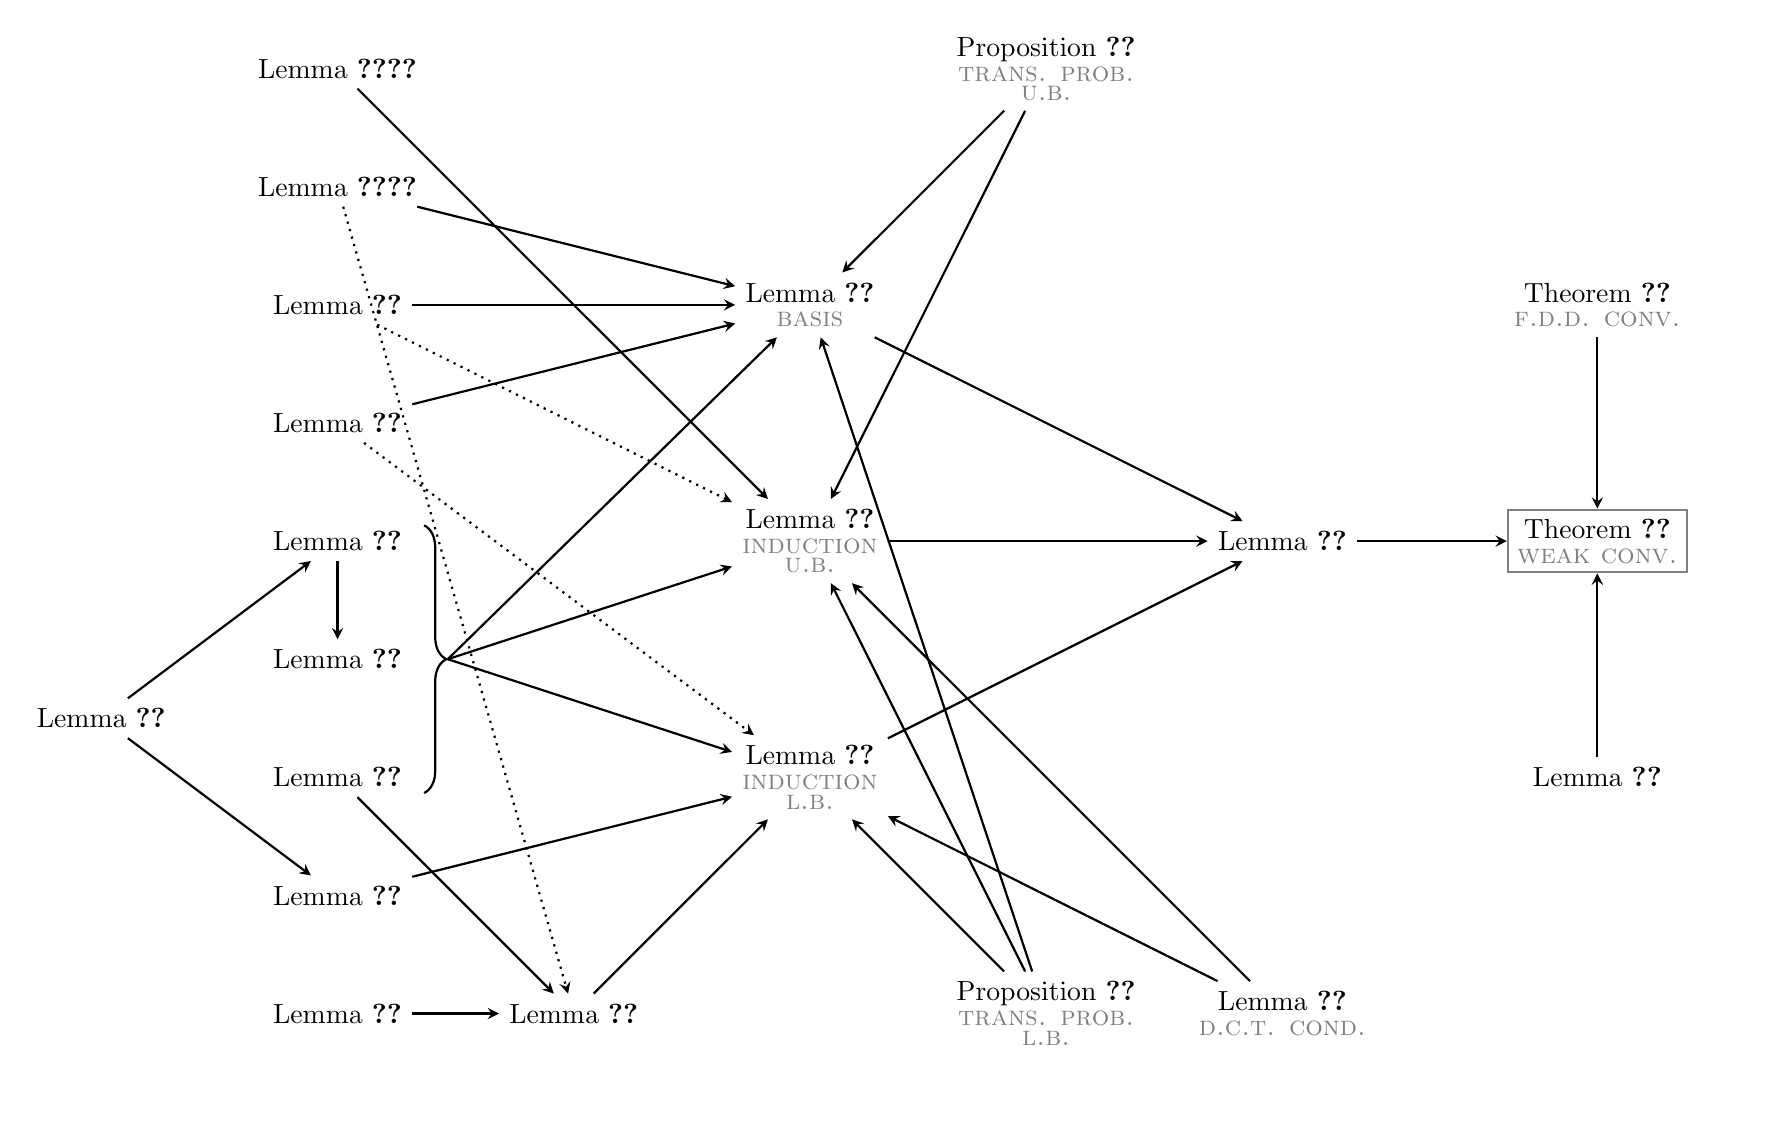
\begin{tikzpicture}[>=stealth, thick]
%% grid lines horizontal
%\draw[gray!20] (-15,0)--(6,0);
%\draw[gray!20] (-15,3)--(6,3);
%\draw[gray!20] (-15,6)--(6,6);
%\draw[gray!20] (-15,-3)--(6,-3);
%\draw[gray!20] (-15,-6)--(6,-6);
%% grid lines vertical
%\draw[gray!20] (0,6)--(0,-6);
%\draw[gray!20] (4,6)--(4,-6);
%\draw[gray!20] (-3,6)--(-3,-6);
%\draw[gray!20] (-6,6)--(-6,-6);
%\draw[gray!20] (-9,6)--(-9,-6);
%\draw[gray!20] (-12,6)--(-12,-6);
%\draw[gray!20] (-15,6)--(-15,-6);

% phantom line (to add space below figure)
\draw[white] (-15,-7)--(6,-7);

% nodes
\node[align=center,draw=gray] at (4,0) (c7r2) 
        {Theorem~\ref{thm:weakconv}\\[-3pt] \textcolor{gray}{\textsc{weak conv.}}};
\node[align=center] at (-6,-3) (c4r3) {Lemma~\ref{thm:inductionLB}\\[-3pt] 
        \textcolor{gray}{\textsc{induction}} \\[-5pt] \textcolor{gray}{\textsc{l.b.}} };
\node[align=center] at (-6,0) (c4r2) {Lemma~\ref{thm:inductionUB}\\[-3pt] 
        \textcolor{gray}{\textsc{induction}} \\[-5pt] \textcolor{gray}{\textsc{u.b.}} };
\node[align=center] at (-6,3) (c4r1) {Lemma~\ref{thm:basis}\\[-3pt] 
        \textcolor{gray}{\textsc{basis}} };
\node[align=center] at (4,3) (c7r1) {Theorem~\ref{thm:FDDconv}\\[-3pt] \textcolor{gray}{\textsc{f.d.d. conv.}} };
\node at (-15,-2.25) (c1r1) {Lemma~\ref{thm:kjjslemma2}};
\node at (4,-3) (c7r3) {Lemma~\ref{thm:maximum_pr}};
\node at (0,0) (c6r1) {Lemma~\ref{thm:holdingtimes_distn}};
\node[align=center] at (-3,6) (c5r1) {Proposition~\ref{thm:pDelta_LB}\\[-3pt] 
        \textcolor{gray}{\textsc{trans. prob.}} \\[-5pt] \textcolor{gray}{\textsc{u.b.}} };
\node[align=center] at (-3,-6) (c5r2) {Proposition~\ref{thm:pDelta_UB}\\[-3pt] 
        \textcolor{gray}{\textsc{trans. prob.}} \\[-5pt] \textcolor{gray}{\textsc{l.b.}} };
\node[align=center] at (0,-6) (c6r2) {Lemma~\ref{thm:DCT_Fubini}\\[-3pt] 
        \textcolor{gray}{\textsc{d.c.t. cond.}} };
\node at (-9,-6) (c3r1) {Lemma~\ref{thm:induction_sumprodcN}};
\node at (-12,6) (c2r1) {Lemma~\ref{thm:sumprod1}\ref{thm:sumprod1_a}};
\node at (-12,4.5) (c2r2) {Lemma~\ref{thm:sumprod1}\ref{thm:sumprod1_b}};
\node at (-12,3) (c2r3) {Lemma~\ref{thm:sumprod2}};
\node at (-12,1.5) (c2r4) {Lemma~\ref{thm:sumprod3}};
\node at (-12,-1.5) (c2r6) {Lemma~\ref{thm:indicators_tau}};
\node at (-12,0) (c2r5) {Lemma~\ref{thm:indicators_cN}};
\node at (-12,-3) (c2r7) {Lemma~\ref{thm:lim_AandB}};
\node at (-12,-4.5) (c2r8) {Lemma~\ref{thm:indicators_DN}};
\node at (-12,-6) (c2r9) {Lemma~\ref{thm:indicators_c2}};

% brace
\draw[decorate, decoration={brace, amplitude=8}] (-10.9,0.2)--(-10.9, -3.2);

% arrows from column 1
\draw[->] (c1r1)--(c2r8);
\draw[->] (c1r1)--(c2r5);
% arrows from column 2
\draw[->] (c2r5)--(c2r6);
\draw[->] (c2r1)--(c4r2);
\draw[->] (c2r2)--(c4r1);
\draw[->, dotted] (c2r2)--(c3r1);
\draw[->] (c2r3)--(c4r1);
\draw[->, dotted] (c2r3)--(c4r2);
\draw[->] (c2r4)--(c4r1);
\draw[->, dotted] (c2r4)--(c4r3);
\draw[->] (c2r8)--(c4r3);
\draw[->] (c2r9)--(c3r1);
\draw[->] (c2r7)--(c3r1);
% arrows from brace
\draw[->] (-10.6, -1.5)--(c4r1);
\draw[->] (-10.6, -1.5)--(c4r2);
\draw[->] (-10.6, -1.5)--(c4r3);
% arrows from column 3
\draw[->] (c3r1)--(c4r3);
% arrows from column 4
\draw[->] (c4r1)--(c6r1);
\draw[->] (c4r2)--(c6r1);
\draw[->] (c4r3)--(c6r1);
% arrows from column 5
\draw[->] (c5r1)--(c4r1);
\draw[->] (c5r1)--(c4r2);
\draw[->] (c5r2)--(c4r1);
\draw[->] (c5r2)--(c4r2);
\draw[->] (c5r2)--(c4r3);
% arrows from column 6
\draw[->] (c6r1)--(c7r2);
\draw[->] (c6r2)--(c4r2);
\draw[->] (c6r2)--(c4r3);
% arrows from column 7
\draw[->] (c7r1)--(c7r2);
\draw[->] (c7r3)--(c7r2);
\end{tikzpicture}
\caption[Structure of weak convergence proof]{Graph showing dependencies between the lemmata used to prove weak convergence. Dotted arrows indicate dependence via a slight modification of the preceding lemma.}
%Dependencies preceding Theorem~\ref{thm:FDDconv} are not shown; these are shown in Figure~??\seb{draw a corresponding figure for fdd proof, or delete this sentence?}.}
\label{fig:weakconv_structure}
\end{figure}
\end{landscape}




\section{Bounds on sum-products}
We start by proving some upper and lower bounds on sums of products of various quantities, which appear from our bounds on $p_r$ (Propositions~\ref{thm:pDelta_LB} and \ref{thm:pDelta_UB}). These sum-product bounds will be applied multiple times in the lemmata of this chapter.

\begin{lemma}\label{thm:sumprod1}
Fix $t>0$, $l\in\mathbb{N}$.
\begin{enumerate}[label=(\alph*)]
\item \label{thm:sumprod1_a} %\hspace{0.2cm}
$\begin{aligned}
\sum_{\substack{ s_1, \dots, s_l =1 \\ \text{\normalfont{all distinct}} }}^{\tau_N(t)}
        \prod_{j=1}^l c_N(s_j)
    \leq (t+1)^l
\end{aligned}$
\item \label{thm:sumprod1_b} %\hspace{0.2cm}
$\begin{aligned}
t^l - \left( \sum_{s=1}^{\tau_N(t)} c_N(s)^2 \right) \binom{l}{2} (t+1)^{l-2} 
    \leq \sum_{\substack{ s_1, \dots, s_l =1 \\ \text{\normalfont{all distinct}} }}
        ^{\tau_N(t)} \prod_{j=1}^l c_N(s_j)
    \leq t^l + c_N(\tau_N(t)) (t+1)^l
\end{aligned}$
\end{enumerate}
\end{lemma}

\begin{proof} \textbf{\ref{thm:sumprod1_a}}
Firstly, we have the inequality
\begin{equation*}
\sum_{\substack{ s_1, \dots, s_l =1 \\ \text{all distinct} }}^{\tau_N(t)}
        \prod_{j=1}^l c_N(s_j)
\leq \left( \sum_{s=0}^{\tau_N(t)} c_N(s) \right)^l ,
\end{equation*}
as can be seen by considering the multinomial expansion of the RHS.
Applying Proposition~\ref{thm:cN_properties}\ref{item:cN_property4},
\begin{equation}\label{eq:039}
\sum_{\substack{ s_1, \dots, s_l =1 \\ \text{all distinct} }}^{\tau_N(t)}
        \prod_{j=1}^l c_N(s_j)
\leq (t+1)^l .
\end{equation}
\textbf{\ref{thm:sumprod1_b}}
As pointed out in \textcite[Equation (8)]{koskela2018}, 
\begin{equation}\label{eq:002}
\sum_{\substack{ s_1, \dots, s_l =1 \\ \text{all distinct} }}^{\tau_N(t)} 
        \prod_{j=1}^l c_N(s_j)
\geq \left( \sum_{s=0}^{\tau_N(t)} c_N(s) \right)^l
        - \binom{l}{2} \left( \sum_{s=0}^{\tau_N(t)} c_N(s)^2 \right)
        \left( \sum_{s=0}^{\tau_N(t)} c_N(s) \right)^{l-2} .
\end{equation}
Applying Proposition~\ref{thm:cN_properties}\ref{item:cN_property4} on the RHS of \eqref{eq:002} yields the lower bound.

For the upper bound we have
\begin{equation*}
\sum_{\substack{ s_1, \dots, s_l =1 \\ \text{all distinct} }}^{\tau_N(t)} 
        \prod_{j=1}^l c_N(s_j)
\leq \left( \sum_{s=0}^{\tau_N(t)} c_N(s) \right)^l
\leq \left( \sum_{s=0}^{\tau_N(t) -1} c_N(s) + c_N(\tau_N(t)) \right)^l
\leq \left[ t + c_N(\tau_N(t)) \right]^l ,
\end{equation*}
using the definition of $\tau_N$.
A binomial expansion yields
\begin{equation*}
\left[ t + c_N(\tau_N(t)) \right]^l
= t^l + \sum_{i=0}^{l-1} \binom{l}{i} t^i c_N(\tau_N(t))^{l-i}
= t^l + c_N(\tau_N(t)) \sum_{i=0}^{l-1} \binom{l}{i} t^i c_N(\tau_N(t))^{l-1-i} ,
\end{equation*}
then by Proposition~\ref{thm:cN_properties}\ref{item:cN_property1},
\begin{equation*}
\sum_{i=0}^{l-1} \binom{l}{i} t^i c_N(\tau_N(t))^{l-1-i}
\leq \sum_{i=0}^{l-1} \binom{l}{i} t^i
\leq (t+1)^l .
\end{equation*}
Putting this together yields the upper bound.
\end{proof}


\begin{lemma}\label{thm:sumprod2}
Fix $t>0$, $l\in\mathbb{N}$.
%Let $B$ be a positive constant which may depend on $n$.
Then, for any constant $B>0$,
\begin{align*}
&\sum_{\substack{ s_1, \dots, s_l =1 \\ \text{\normalfont{all distinct}} }}^{\tau_N(t)} 
        \prod_{j=1}^l \left[ c_N(s_j) + B D_N(s_j) \right] \\
&\hspace{4cm}\leq \sum_{\substack{ s_1, \dots, s_l =1 \\ \text{\normalfont{all distinct}} }}^{\tau_N(t)} 
        \prod_{j=1}^l c_N(s_j)
        + \left( \sum_{s=1}^{\tau_N(t)} D_N(s) \right) (t+1)^{l-1} (1+B)^l .
\end{align*}
\end{lemma}

\begin{proof}
We start with a binomial expansion:
\begin{align}
\sum_{\substack{ s_1, \dots, s_l =1 \\ \text{all distinct} }}^{\tau_N(t)} 
        \prod_{j=1}^l \left[ c_N(s_j) + B D_N(s_j) \right]
&= \sum_{\substack{ s_1, \dots, s_l =1 \\ \text{all distinct} }}^{\tau_N(t)} 
        \sum_{\mathcal{I} \subseteq [l]}
        B^{l-|\mathcal{I}|} \left( \prod_{i\in\mathcal{I}} c_N(s_i) \right)
        \left( \prod_{j\notin\mathcal{I}} D_N(s_j) \right) \notag\\
&= \sum_{\mathcal{I} \subseteq [l]} B^{l-|\mathcal{I}|}
        \sum_{\substack{ s_1, \dots, s_l =1 \\ \text{all distinct} }}^{\tau_N(t)}
        \left( \prod_{i\in\mathcal{I}} c_N(s_i) \right)
        \left( \prod_{j\notin\mathcal{I}} D_N(s_j) \right) \label{eq:010}
\end{align}
where $[l] := \{1,\dots,l\}$. Since we are summing over all permutations of $s_1,\dots,s_l$, the particular partition of $\{1,\dots,l\}$ into $(\mathcal{I},\mathcal{I}^c)$ is not important; only the size of $\mathcal{I}$ matters. We may therefore replace the sum over $\mathcal{I}$ with a sum over $I:= |\mathcal{I}|$ and, without loss of generality, set $\mathcal{I} = \{1,\dots,I\}$:
%we may arbitrarily choose an ordering for $\{1,\dots,l\}$ such that $\mathcal{I} = \{ 1,\dots, |\mathcal{I}| \}$:
\begin{align*}
\sum_{\mathcal{I} \subseteq [l]} B^{l-|\mathcal{I}|}
        \sum_{\substack{ s_1, \dots, s_l =1 \\ \text{all distinct} }}^{\tau_N(t)}
        &\left( \prod_{i\in\mathcal{I}} c_N(s_i) \right)
        \left( \prod_{j\notin\mathcal{I}} D_N(s_j) \right) \\
&= \sum_{I=0}^l \binom{l}{I} B^{l-I} 
        \sum_{\substack{ s_1, \dots, s_l =1 \\ \text{all distinct} }}^{\tau_N(t)}
        \left( \prod_{i=1}^I c_N(s_i) \right)
        \left( \prod_{j=I+1}^l D_N(s_j) \right) .
\end{align*}
Separating the term $I=l$,
\begin{align}
\sum_{I=0}^l \binom{l}{I} &B^{l-I} 
        \sum_{\substack{ s_1, \dots, s_l =1 \\ \text{all distinct} }}^{\tau_N(t)}
        \left( \prod_{i=1}^I c_N(s_i) \right)
        \left( \prod_{j=I+1}^l D_N(s_j) \right) \notag\\
&= \sum_{\substack{ s_1, \dots, s_l =1 \\ \text{all distinct} }}^{\tau_N(t)}
        \prod_{j=1}^l c_N(s_j)
    + \sum_{I=0}^{l-1} \binom{l}{I} B^{l-I} 
        \sum_{\substack{ s_1, \dots, s_l =1 \\ \text{all distinct} }}^{\tau_N(t)}
        \left( \prod_{i=1}^I c_N(s_i) \right) \left( \prod_{j=I+1}^l D_N(s_j) \right). \label{eq:012}
\end{align}
In the second term on the RHS, there is always at least one $D_N$ term, so using Proposition~\ref{thm:cN_properties}\ref{item:cN_property2} we can write
\begin{align}
\sum_{I=0}^{l-1}\binom{l}{I} B^{l-I} 
        &\sum_{\substack{ s_1, \dots, s_l =1 \\ \text{all distinct} }}^{\tau_N(t)}
        \left( \prod_{i=1}^I c_N(s_i) \right) \left( \prod_{j=I+1}^l D_N(s_j) \right) \notag\\
&\leq \sum_{I=0}^{l-1}\binom{l}{I} B^{l-I} 
        \sum_{\substack{ s_1, \dots, s_l =1 \\ \text{all distinct} }}^{\tau_N(t)}
        \left( \prod_{i=1}^{l-1} c_N(s_i) \right) D_N(s_l) \notag\\
&\leq \sum_{I=0}^{l-1}\binom{l}{I} B^{l-I} 
        \left( \sum_{\substack{ s_1, \dots, s_l =1 \\ \text{all distinct} }}^{\tau_N(t)}
        \prod_{i=1}^{l-1} c_N(s_i) \right) 
        \sum_{s_l=1}^{\tau_N(t)} D_N(s_l) \notag\\
&\leq \sum_{I=0}^{l-1}\binom{l}{I} B^{l-I} (t+1)^{l-1}
        \sum_{s=1}^{\tau_N(t)} D_N(s) \label{eq:013}
\end{align}
using \eqref{eq:039}.
Finally, by the Binomial Theorem,
\begin{equation}\label{eq:014}
\sum_{I=0}^{l-1}\binom{l}{I} B^{l-I} (t+1)^{l-1}
        \sum_{s=1}^{\tau_N(t)} D_N(s)
\leq \left( \sum_{s=1}^{\tau_N(t)} D_N(s) \right) (t+1)^{l-1} (1+B)^l ,
\end{equation}
which, together with \eqref{eq:012}, concludes the proof.
\end{proof}


\begin{lemma}\label{thm:sumprod3}
Fix $t>0$, $l\in\mathbb{N}$.
%Let $B$ be a positive constant which may depend on $n$.
Then, for any constant $B>0$,
\begin{align*}
&\sum_{\substack{ s_1, \dots, s_l =1 \\ \text{\normalfont{all distinct}} }}^{\tau_N(t)} 
        \prod_{j=1}^l \left[ c_N(s_j) - B D_N(s_j) \right] \\
&\hspace{4cm}\geq \sum_{\substack{ s_1, \dots, s_l =1 \\ \text{\normalfont{all distinct}} }}^{\tau_N(t)} 
        \prod_{j=1}^l c_N(s_j)
        - \left( \sum_{s=1}^{\tau_N(t)} D_N(s) \right) (t+1)^{l-1} (1+B)^l .
\end{align*}
\end{lemma}

\begin{proof}
A binomial expansion and subsequent manipulation as in \eqref{eq:010}--\eqref{eq:012} gives
\begin{align*}
\sum_{\substack{ s_1, \dots, s_l =1 \\ \text{all distinct} }}^{\tau_N(t)} 
        &\prod_{j=1}^l 
        \left[ c_N(s_j) - B D_N(s_j) \right] \\
&= \sum_{\mathcal{I} \subseteq [l]} (-B)^{l-|\mathcal{I}|}
        \sum_{\substack{ s_1, \dots, s_l =1 \\ \text{all distinct} }}^{\tau_N(t)}
        \left( \prod_{i\in\mathcal{I}} c_N(s_i) \right)
        \left( \prod_{j\notin\mathcal{I}} D_N(s_j) \right) \\
&= \sum_{I=0}^l \binom{l}{I} (-B)^{l-I} 
        \sum_{\substack{ s_1, \dots, s_l =1 \\ \text{all distinct} }}^{\tau_N(t)}
        \left( \prod_{i=1}^I c_N(s_i) \right)
        \left( \prod_{j=I+1}^l D_N(s_j) \right) \\
&= \sum_{\substack{ s_1, \dots, s_l =1 \\ \text{all distinct} }}^{\tau_N(t)} 
        \prod_{j=1}^l c_N(s_j)
        + \sum_{I=0}^{l-1} \binom{l}{I} (-B)^{l-I} 
        \sum_{\substack{ s_1, \dots, s_l =1 \\ \text{all distinct} }}^{\tau_N(t)}
        \left( \prod_{i=1}^I c_N(s_i) \right) 
        \left( \prod_{j=I+1}^l D_N(s_j) \right) \\
&\geq \sum_{\substack{ s_1, \dots, s_l =1 \\ \text{all distinct} }}^{\tau_N(t)} 
        \prod_{j=1}^l c_N(s_j)
        - \sum_{I=0}^{l-1} \binom{l}{I} B^{l-I} 
        \sum_{\substack{ s_1, \dots, s_l =1 \\ \text{all distinct} }}^{\tau_N(t)}
        \left( \prod_{i=1}^I c_N(s_i) \right) \left( \prod_{j=I+1}^l D_N(s_j) \right)
\end{align*}
where the last inequality just multiplies some positive terms by $-1$.
Then \eqref{eq:013}--\eqref{eq:014} can be applied directly (noting that an upper bound on negative terms gives a lower bound overall):
\begin{align*}
&- \sum_{I=0}^{l-1} \binom{l}{I} B^{l-I} 
        \sum_{\substack{ s_1, \dots, s_l =1 \\ \text{all distinct} }}^{\tau_N(t)}
        \left( \prod_{i=1}^I c_N(s_i) \right) \left( \prod_{j=I+1}^l D_N(s_j) \right) \\
&\hspace{2cm}\geq - \left( \sum_{s=1}^{\tau_N(t)} D_N(s) \right) (t+1)^{l-1} (1+B)^l 
\end{align*}
which concludes the proof.
\end{proof}




\section{Main components of induction argument}
This section contains the technical aspects of the proof of Lemma~\ref{thm:holdingtimes_distn}, which establishes the limiting distributions of holding times of the coupled process, via an induction argument.
This section is split into four lemmata: the first (Lemma~\ref{thm:basis}) is used in the basis step and the others in the induction step. The induction step is established by combining upper and lower bounds, proved in Lemmata~\ref{thm:inductionUB} and \ref{thm:inductionLB} respectively. Lemma~\ref{thm:induction_sumprodcN} is a technical result which is common to both the upper and lower bounds, determining the limit as $N\to\infty$ of a certain expectation that arises in both bounds.

Recall that the following conditions are all consequences of \eqref{eq:mainthmcondition2}: for all $t>s>0$,
\begin{align}
\E \left[ c_N(\tau_N(t)) \right] &\rightarrow 0 \label{eq:BJJK_eq3.3}\\
\E\left[ \sum_{r=\tau_N(s)+1}^{\tau_N(t)} c_N(r)^2 \right] &\rightarrow 0
        \label{eq:BJJK_eq3.5}\\
\E\left[ \sum_{r=\tau_N(s)+1}^{\tau_N(t)} D_N(r) \right] &\rightarrow 0
        \label{eq:BJJK_eq3.4}
\end{align}
as $N\to\infty$. (See Lemmata~\ref{lem:removeass3}, \ref{thm:DNimpliescN} and \ref{lem:removeass2} for proofs.)
%Also recall the following properties from Proposition~\ref{thm:cN_properties}:
%\begin{align}
%& c_N(t) , D_N(t) \in [0,1] \label{eq:cN_property1}\\
%& D_N(t) \leq c_N(t) \label{eq:cN_property2}\\
%& t^\prime
%    \leq \sum_{r=1}^{\tau_N(t^\prime)} c_N(r) 
%    \leq t^\prime +1 .\label{eq:cN_property4}
%\end{align}



\begin{lemma}[Basis step]\label{thm:basis}
Assume \eqref{eq:mainthmcondition2} holds.
For any $0 < t < \infty$,
\begin{equation*}
\lim_{N\to\infty} \E\left[ \prod_{r=1}^{\tau_N(t)} (1-p_r) \right] 
= e^{-\alpha_n t}
\end{equation*}
where $\alpha_n := n(n-1)/2$.
\end{lemma}

\begin{proof}
We start by showing that
$\lim_{N\to\infty}\E\left[ \prod_{r=1}^{\tau_N(t)} (1-p_r) \right] 
\leq e^{-\alpha_n t}$.\\
Setting $\xi=\Delta$ in Proposition~\ref{thm:pDelta_UB}, we have for each $r$ and for sufficiently large $N$
\begin{equation} \label{eq:018}
1-p_r
= p_{\Delta\Delta}(r) 
\leq 1 - \alpha_n \ON % \frac{N^{n-2}}{(N-2)_{n-2}}
        \left[ c_N(r) - B_n^\prime D_N(r) \right] .
\end{equation}
%\seb{Explain why we need the indicators... bounds only valid for large enough $N$... may go negative for some values of $N$... product of negative bounds could be problematic... but don't we only care about the large-$N$ regime in which these bounds are valid (and therefore must be non-negative) and everything is fine...?}\\
Since we will eventually take $N\to\infty$, it is sufficient to have bounds that hold for large enough $N$. However, some of the manipulations below require that these bounds are non-negative. For this reason we introduce some indicator functions (which will be almost surely equal to $1$ in the limit) to keep the bounds non-negative.
These indicators will later be dropped from certain terms that are clearly non-negative without them. 
The indicators introduced at this point are such that if their conditions do not hold then the bound becomes the trivial $1-p_r \leq 1$.
 
When $N \geq 3$, a sufficient condition to ensure the bound in \eqref{eq:018} is non-negative is that the event
\begin{equation}\label{eq:defn_E1}
E_N^{1}(r) := \left\{ c_N(r) < \alpha_n^{-1} A_N \right\} 
\end{equation}
occurs, where $A_N = \ON$ as $N\to\infty$ and is independent of $r$ but will not be specified explicitly.
We will also need to control the sign of $c_N(r) - B_n^\prime D_N(r)$, for which we define the event
\begin{equation}\label{eq:defn_E2}
E_N^2(r) := \left\{ c_N(r) \geq B_n^\prime D_N(r) \right\} ,
\end{equation}
and we define $E_N^1 := \bigcap_{r=1}^{\tau_N(t)} E_N^1(r)$ and $E_N^2 := \bigcap_{r=1}^{\tau_N(t)} E_N^2(r)$.
Then
\begin{equation*}
1-p_r
= p_{\Delta\Delta}(r) \leq 1 - \alpha_n \ON 
        \left[ c_N(r) - B_n^\prime D_N(r) \right] \1{E_N^1 \cap E_N^2} .
\end{equation*}
Applying a multinomial expansion and then separating the positive and negative terms,
\begin{align}
\prod_{r=1}^{\tau_N(t)} (1-p_r)
&\leq 1 + \sum_{l=1}^{\tau_N(t)} (- \alpha_n)^l \ON 
        \frac{1}{l!} \sum_{\substack{ s_1, \dots, s_l =1 \\ \text{all distinct} }}^{\tau_N(t)}
        \prod_{j=1}^l
        \left[ c_N(s_j) - B_n^\prime D_N(s_j) \right] \1{E_N^1 \cap E_N^2} \notag\\
&= 1 + \sum_{\substack{l=2 \\ \text{even} }}^{\tau_N(t)} 
        \alpha_n^l \ON \frac{1}{l!} 
        \sum_{\substack{ s_1, \dots, s_l =1 \\ \text{all distinct} }}^{\tau_N(t)}
        \prod_{j=1}^l
        \left[ c_N(s_j) - B_n^\prime D_N(s_j) \right] \1{E_N^1 \cap E_N^2} \notag\\
    &\qquad- \sum_{\substack{l=1 \\ \text{odd} }}^{\tau_N(t)} 
        \alpha_n^l \ON \frac{1}{l!} 
        \sum_{\substack{ s_1, \dots, s_l =1 \\ \text{all distinct} }}^{\tau_N(t)}
        \prod_{j=1}^l
        \left[ c_N(s_j) - B_n^\prime D_N(s_j) \right] \1{E_N^1 \cap E_N^2} .
        \label{eq:019}
\end{align}
This is further bounded by applying Lemma~\ref{thm:sumprod3} and then both bounds of Lemma~\ref{thm:sumprod1}\ref{thm:sumprod1_b}:
\begin{align*}
&\prod_{r=1}^{\tau_N(t)} (1-p_r) \\
&\quad\leq 1 + \1{E_N^1 \cap E_N^2} \Bigg\{ 
        \sum_{\substack{l=2 \\ \text{even} }}^{\tau_N(t)} 
        \alpha_n^l \ON \frac{1}{l!} 
        \sum_{\substack{ s_1, \dots, s_l =1 \\ \text{all distinct} }}^{\tau_N(t)}
        \prod_{j=1}^l c_N(s_j) \\
    &\qquad- \sum_{\substack{l=1 \\ \text{odd} }}^{\tau_N(t)} 
        \alpha_n^l \ON \frac{1}{l!} 
        \left[ \sum_{\substack{ s_1, \dots, s_l =1 \\ \text{all distinct} }}^{\tau_N(t)}
        \prod_{j=1}^l c_N(s_j)
        - \left( \sum_{s=1}^{\tau_N(t)} D_N(s) \right) 
        (t+1)^{l-1} (1+B_n^\prime)^l \right] \Bigg\} \\
&\quad\leq 1 + \Bigg\{ \sum_{\substack{l=2 \\ \text{even} }}^{\tau_N(t)} 
        \alpha_n^l \ON \frac{1}{l!} 
        \left\{ t^l + c_N(\tau_N(t)) (t+1)^l \right\} \\
    &\qquad- \sum_{\substack{l=1 \\ \text{odd} }}^{\tau_N(t)} 
        \alpha_n^l \ON \frac{1}{l!} 
        \left[ t^l - \left( \sum_{s=1}^{\tau_N(t)} c_N(s)^2 \right) 
        \binom{l}{2} (t+1)^{l-2} \right] \\
    &\qquad- \left( \sum_{s=1}^{\tau_N(t)} D_N(s) \right) 
        (t+1)^{l-1} (1+B_n^\prime)^l \Bigg\} \1{E_N^1 \cap E_N^2} .
\end{align*}
Collecting some terms,
\begin{align}
\prod_{r=1}^{\tau_N(t)} (1-p_r)
&\leq 1+ \sum_{l=1}^{\tau_N(t)} (-\alpha_n)^l \ON \frac{1}{l!} t^l 
        \1{E_N^1 \cap E_N^2}
        + c_N(\tau_N(t)) \sum_{\substack{l=2 \\ \text{even} }}^{\tau_N(t)}
        \alpha_n^l \ON \frac{1}{l!} (t+1)^l \notag\\
    &\qquad+ \left( \sum_{s=1}^{\tau_N(t)} c_N(s)^2 \right)
        \sum_{\substack{l=1 \\ \text{odd} }}^{\tau_N(t)} \alpha_n^l
        \ON \frac{1}{l!} \binom{l}{2} (t+1)^{l-2} \notag\\
    &\qquad+ \left( \sum_{s=1}^{\tau_N(t)} D_N(s) \right) 
        \sum_{\substack{l=1 \\ \text{odd} }}^{\tau_N(t)} \alpha_n^l
        \ON \frac{1}{l!} (t+1)^{l-1} (1+B_n^\prime)^l \notag\\
&\leq 1+ \sum_{l=1}^{\infty} (-\alpha_n)^l \ON \frac{1}{l!} t^l
        \I{\tau_N(t) \geq l} \1{E_N^1 \cap E_N^2}
        + c_N(\tau_N(t)) \exp[ \alpha_n \ON (t+1) ] \notag\\
    &\qquad+ \left( \sum_{s=1}^{\tau_N(t)} c_N(s)^2 \right)
        \frac{1}{2} \alpha_n^2 \exp[ \alpha_n \ON (t+1) ] \notag\\
    &\qquad+ \left( \sum_{s=1}^{\tau_N(t)} D_N(s) \right)
        \exp[ \alpha_n \ON (t+1) (1+B_n^\prime) ] . \label{eq:021}
\end{align}
The requirement $\tau_N(t) \geq l$ has been dropped in the second term because the additional terms there are all positive and we only need an upper bound.
Now, taking the expectation and limit, then applying \eqref{eq:BJJK_eq3.3}--\eqref{eq:BJJK_eq3.4}, and Lemmata \ref{thm:indicators_cN}, \ref{thm:indicators_tau} and \ref{thm:indicators_DN} to deal with the indicators,
\begin{align}
\lim_{N\to\infty} \E \left[ \prod_{r=1}^{\tau_N(t)} (1-p_r) \right]
&\leq 1+ \sum_{l=1}^{\infty} (-\alpha_n)^l \frac{1}{l!} t^l
        \lim_{N\to\infty} \Prob \left[ \{\tau_N(t) \geq l\} \cap E_N^1 \cap E_N^2 \right] \notag\\
    &\qquad+ \lim_{N\to\infty} \E \left[ c_N(\tau_N(t)) \right]
        \exp[ \alpha_n (t+1) ] \notag\\
    &\qquad+ \lim_{N\to\infty} \E \left[ \sum_{s=1}^{\tau_N(t)} 
        c_N(s)^2 \right]
        \frac{1}{2} \alpha_n^2 \exp[ \alpha_n (t+1) ] \notag\\
    &\qquad+ \lim_{N\to\infty} \E \left[ \sum_{s=1}^{\tau_N(t)} D_N(s) \right]
        \exp[ \alpha_n (t+1) (1+B_n^\prime) ] \notag\\
&= 1+ \sum_{l=1}^{\infty} (-\alpha_n)^l \frac{1}{l!} t^l
= e^{-\alpha_n t}. \label{eq:022}
\end{align}
Passing the limit and expectation inside the infinite sum is justified by dominated convergence and Fubini.

It remains to show the corresponding lower bound
\begin{equation*}
    \lim_{N\to\infty} \E\left[ \prod_{r=1}^{\tau_N(t)} (1-p_r) \right] 
\geq e^{-\alpha_n t} .
\end{equation*}
Setting $\xi=\Delta$ in Proposition~\ref{thm:pDelta_LB}, we have
\begin{equation}\label{eq:pDeltaDelta_LB}
1-p_t
= p_{\Delta\Delta}(t) \geq 1 - \frac{N^{n-2}}{(N-2)_{n-2}} \alpha_n 
    [ c_N(t) + B_n D_N(t) ] 
\end{equation}
where $B_n >0$.
Due to Proposition~\ref{thm:cN_properties}\eqref{item:cN_property2}, a sufficient condition for this bound to be non-negative is
\begin{equation}\label{eq:defn_E3}
E_N^3(r)
:= \left\{ c_N(r) \leq \frac{(N-2)_{n-2}}{N^{n-2}} 
        \alpha_n^{-1} (1+B_n)^{-1} \right\} ,
\end{equation}
and we again define $E_N^3 := \bigcap_{r=1}^{\tau_N(t)} E_N^3(r)$.
We now apply a multinomial expansion to the product, and split into positive and negative terms:
\begin{align*}
\prod_{r=1}^{\tau_N(t)} (1-p_r)
&\geq \left\{ 1 + \sum_{l=1}^{\tau_N(t)} (-\alpha_n)^l \ON 
        \frac{1}{l!} \sum_{\substack{ s_1, \dots, s_l =1 \\ \text{all distinct} }}^{\tau_N(t)}
        \prod_{j=1}^l
        \left[ c_N(s_j) + B_n D_N(s_j) \right] \right\} \1{E_N^3} \\
&= \Bigg\{ 1 + \sum_{\substack{l=2 \\ \text{even} }}^{\tau_N(t)} 
        \alpha_n^l \ON \frac{1}{l!} 
        \sum_{\substack{ s_1, \dots, s_l =1 \\ \text{all distinct} }}^{\tau_N(t)}
        \prod_{j=1}^l
        \left[ c_N(s_j) + B_n D_N(s_j) \right] \\
    &\qquad- \sum_{\substack{l=1 \\ \text{odd} }}^{\tau_N(t)} 
        \alpha_n^l \ON \frac{1}{l!}
        \sum_{\substack{ s_1, \dots, s_l =1 \\ \text{all distinct} }}^{\tau_N(t)}
        \prod_{j=1}^l
        \left[ c_N(s_j) + B_n D_N(s_j) \right] \Bigg\} \1{E_N^3}
\end{align*}
This is further bounded by applying Lemma~\ref{thm:sumprod2} and both bounds in Lemma~\ref{thm:sumprod1}\ref{thm:sumprod1_b}:
\begin{align*}
&\prod_{r=1}^{\tau_N(t)} (1-p_r) \\
&\quad\geq \1{E_N^3} \Bigg\{ 1 + 
        \sum_{\substack{l=2 \\ \text{even} }}^{\tau_N(t)} 
        \alpha_n^l \ON \frac{1}{l!} 
        \sum_{\substack{ s_1, \dots, s_l =1 \\ \text{all distinct} }}^{\tau_N(t)}
        \prod_{j=1}^l c_N(s_j) \\
    &\qquad- \sum_{\substack{l=1 \\ \text{odd} }}^{\tau_N(t)} 
        \alpha_n^l \ON \frac{1}{l!}
        \left[ \sum_{\substack{ s_1, \dots, s_l =1 \\ \text{all distinct} }}^{\tau_N(t)}
        \prod_{j=1}^l c_N(s_j)
        + \left( \sum_{s=1}^{\tau_N(t)} D_N(s) \right)
        (t+1)^{l-1} (1+B_n)^l \right] \Bigg\} \\
&\quad\geq \1{E_N^3} \Bigg\{ 1 + 
        \sum_{\substack{l=2 \\ \text{even} }}^{\tau_N(t)} 
        \alpha_n^l \ON \frac{1}{l!} 
        \left[ t^l - \left( \sum_{s=1}^{\tau_N(t)} c_N(s)^2 \right)
        \binom{l}{2}(t+1)^{l-2} \right] \\
    &\qquad- \sum_{\substack{l=1 \\ \text{odd} }}^{\tau_N(t)} 
        \alpha_n^l \ON \frac{1}{l!}
        \left[ t^l + c_N(\tau_N(t)) (t+1)^l
        + \left( \sum_{s=1}^{\tau_N(t)} D_N(s) \right)
        (t+1)^{l-1} (1+B_n)^l \right] \Bigg\} .
\end{align*}
Collecting terms,
\begin{align}
\prod_{r=1}^{\tau_N(t)} (1-p_r)
&\geq \sum_{l=0}^{\tau_N(t)} (-\alpha_n)^l \ON 
        \frac{1}{l!} t^l \1{E_N^3}
        - \left( \sum_{s=1}^{\tau_N(t)} c_N(s)^2 \right)
        \sum_{\substack{l=2 \\ \text{even} }}^{\tau_N(t)} 
        \alpha_n^l \ON \frac{1}{l!} \binom{l}{2}(t+1)^{l-2} \notag\\
    &\qquad- c_N(\tau_N(t)) \sum_{\substack{l=1 \\ \text{odd} }}^{\tau_N(t)} 
        \alpha_n^l \ON \frac{1}{l!} (t+1)^l \notag\\
    &\qquad- \left( \sum_{s=1}^{\tau_N(t)} D_N(s) \right)
        \sum_{\substack{l=1 \\ \text{odd} }}^{\tau_N(t)} 
        \alpha_n^l \ON \frac{1}{l!} (t+1)^{l-1} (1+B_n)^l \notag\\
&\geq \sum_{l=0}^{\infty} (-\alpha_n)^l \ON 
        \frac{1}{l!} t^l \1{E_N^3} \I{ \tau_N(t) \geq l}
        - \left( \sum_{s=1}^{\tau_N(t)} c_N(s)^2 \right)
        \frac{1}{2} \alpha_n^2 \exp[ \alpha_n \ON (t+1) ]\notag\\
    &\qquad- c_N(\tau_N(t)) \exp[ \alpha_n \ON (t+1) ] \notag\\
    &\qquad- \left( \sum_{s=1}^{\tau_N(t)} D_N(s) \right)
        \exp[ \alpha_n \ON (t+1) (1+B_n) ]. \label{eq:028}
\end{align}
Now, taking the expectation and limit, and applying \eqref{eq:BJJK_eq3.3}--\eqref{eq:BJJK_eq3.4} to show that all but the first sum vanish, and Lemmata~\ref{thm:indicators_cN} and \ref{thm:indicators_tau} to show that $\lim_{N\to\infty} \Prob[ \{\tau_N(t) \geq l\} \cap E_N^3 ] =1$,
\begin{align}
\lim_{N\to\infty} \E \left[ \prod_{r=1}^{\tau_N(t)} (1-p_r) \right]
&\geq \sum_{l=0}^{\infty} (-\alpha_n)^l \ON \frac{1}{l!} t^l 
        \lim_{N\to\infty} \Prob\left[ \{\tau_N(t) \geq l\} \cap E_N^3 \right] \notag\\
    &\qquad- \lim_{N\to\infty} \E \left[ \sum_{s=1}^{\tau_N(t)} c_N(s)^2 \right]
        \frac{1}{2} \alpha_n^2 \exp[ \alpha_n (t+1) ]\notag\\
    &\qquad- \lim_{N\to\infty} \E \left[ c_N(\tau_N(t)) \right] 
        \exp[ \alpha_n (t+1) ] \notag\\
    &\qquad- \lim_{N\to\infty} \E \left[ \sum_{s=1}^{\tau_N(t)} D_N(s) \right]
        \exp[ \alpha_n (t+1) (1+B_n) ] \notag\\
&= \sum_{l=0}^{\infty} (-\alpha_n)^l \frac{1}{l!} t^l
= e^{-\alpha_n t}. \label{eq:029}
\end{align}
Again, passing the limit and expectation inside the infinite sum is justified by dominated convergence and Fubini.
Combining the upper and lower bounds in \eqref{eq:022} and \eqref{eq:029} respectively concludes the proof.
\end{proof}



\begin{lemma}[Induction step upper bound]\label{thm:inductionUB}
Assume \eqref{eq:mainthmcondition2} holds.
Fix $k \in \mathbb{N}$, $i_0:=0$, $i_k:=k$. For any sequence of times
$0 = t_0 \leq t_1 \leq \cdots \leq t_k \leq t$,
\begin{align*}
&\lim_{N\to\infty} \E \left[ 
        \sum_{\substack{r_1 <\dots< r_k :\\ r_i \leq \tau_N(t_i) \forall i}}
        \left( \prod_{i=1}^k p_{r_i} \right)
        \left( \prod_{\substack{r=1 \\ \notin \{r_1,\dots,r_k\} }}^{\tau_N(t)} 
        (1-p_r) \right) \right] \\
&\hspace{6cm}\leq \alpha_n^k e^{-\alpha_n t}
        \sum_{\substack{i_1\leq \dots\leq i_{k-1}\\ \in \{0,\dots,k\} :
        \\ i_j \geq j \forall j}} 
        \prod_{j=1}^k \frac{(t_j - t_{j-1})^{i_j - i_{j-1}}}{(i_j - i_{j-1})! } .
\end{align*}
\end{lemma}

\begin{proof}
We use the bound on $(1-p_r)$ from \eqref{eq:018}, which holds for sufficiently large $N$, and apply a multinomial expansion. Define as in \eqref{eq:defn_E1} and \eqref{eq:defn_E2} respectively the sequences of events $E_N^1$ and $E_N^2$ which keep the bounds non-negative for all $N\geq 3$ so that the following manipulations make sense:
\begin{align}
\prod_{\substack{r=1 \\ \notin \{r_1,\dots,r_k\} }}^{\tau_N(t)} (1-p_r)
&\leq \prod_{\substack{r=1 \\ \notin \{r_1,\dots,r_k\} }}^{\tau_N(t)} 
        \left\{ 1 - \alpha_n  \ON [ c_N(r) - B_n^\prime D_N(r) ] 
        \1{E_N^1 \cap E_N^2} \right\} \notag\\
&= 1 + \sum_{l=1}^{\tau_N(t) -k}
        (-\alpha_n)^l \ON \frac{1}{l!}
        \sum_{\substack{s_1, \dots, s_l =1 \\ \notin \{r_1,\dots,r_k\} 
        \\ \text{all distinct} }}^{\tau_N(t)}
        \prod_{j=1}^l [ c_N(s_j) - B_n^\prime D_N(s_j) ]
        \1{E_N^1 \cap E_N^2} \notag\\
&= 1 + \sum_{l=1}^{\tau_N(t) -k}
        (-\alpha_n)^l \ON \frac{1}{l!}
        \sum_{\substack{ s_1, \dots, s_l =1 \\ \text{all distinct} }}^{\tau_N(t)}
        \prod_{j=1}^l [ c_N(s_j) - B_n^\prime D_N(s_j) ] \1{E_N^1 \cap E_N^2} \notag\\
    &\qquad- \sum_{l=1}^{\tau_N(t) -k}
        (-\alpha_n)^l \ON \frac{1}{l!}
        \sum_{\substack{s_1, \dots, s_l =1 \\ \text{all distinct}: 
        \\ \exists i,i^\prime : s_i=r_{i^\prime} }}^{\tau_N(t)} 
        \prod_{j=1}^l [ c_N(s_j) - B_n^\prime D_N(s_j) ]
        \1{E_N^1 \cap E_N^2} . \label{eq:031}
\end{align}
The penultimate line above is exactly the expansion we had in the basis step \eqref{eq:019}, except for the limit on $l$, and as such following the same arguments gives a bound analogous to that in \eqref{eq:021}:
\begin{align*}
1 + \sum_{l=1}^{\tau_N(t) -k}
        (-\alpha_n)^l \ON \frac{1}{l!}
        &\sum_{\substack{ s_1, \dots, s_l =1 \\ \text{all distinct} }}^{\tau_N(t)}
        \prod_{j=1}^l [ c_N(s_j) - B_n^\prime D_N(s_j) ] \1{E_N^1 \cap E_N^2} \\
&\leq 1+ \sum_{l=1}^{\tau_N(t) -k} (-\alpha_n)^l \ON \frac{1}{l!} t^l
        \1{E_N^1 \cap E_N^2}
        + c_N(\tau_N(t)) \exp[ \alpha_n \ON (t+1) ] \\
    &\qquad+ \left( \sum_{s=1}^{\tau_N(t)} c_N(s)^2 \right)
        \frac{1}{2} \alpha_n^2 \exp[ \alpha_n \ON (t+1) ] \\
    &\qquad+ \left( \sum_{s=1}^{\tau_N(t)} D_N(s) \right)
        \exp[ \alpha_n \ON (t+1) (1+B_n^\prime) ] .
\end{align*}
For the last line of \eqref{eq:031}, recalling that $D_N(t) \leq c_N(t)$ (Proposition~\ref{thm:cN_properties}\ref{item:cN_property2}),
\begin{align*}
- \sum_{l=1}^{\tau_N(t) -k} (-\alpha_n)^l &\ON \frac{1}{l!}
        \sum_{\substack{s_1, \dots, s_l =1 \\ \text{all distinct}: 
        \\ \exists i,i^\prime : s_i=r_{i^\prime} }}^{\tau_N(t)} 
        \prod_{j=1}^l \{ c_N(s_j) - B_n^\prime D_N(s_j) \} 
        \1{E_N^1 \cap E_N^2} \\
&\leq \sum_{l=1}^{\tau_N(t) -k} \alpha_n^l \ON \frac{1}{l!}
        \sum_{\substack{s_1, \dots, s_l =1 \\ \text{all distinct}: 
        \\ \exists i,i^\prime : s_i=r_{i^\prime} }}^{\tau_N(t)} 
        \prod_{j=1}^l \{ c_N(s_j) + B_n^\prime D_N(s_j) \} \\
&\leq \sum_{l=1}^{\tau_N(t) -k} \alpha_n^l \ON \frac{1}{l!}
        \sum_{\substack{s_1, \dots, s_l =1 \\ \text{all distinct}: 
        \\ \exists i,i^\prime : s_i=r_{i^\prime} }}^{\tau_N(t)} 
        (1 + B_n^\prime)^l \prod_{j=1}^l c_N(s_j) \\
&\leq \sum_{l=1}^{\tau_N(t) -k} \alpha_n^l \ON
        \frac{1}{(l-1)!} \sum_{s_1 \in \{r_1,\dots,r_k\} } 
        \sum_{\substack{ s_2, \dots, s_l =1 \\ \text{all distinct} }}^{\tau_N(t)}
        (1 + B_n^\prime)^l \prod_{j=1}^l c_N(s_j) \\
&= \sum_{s \in \{r_1,\dots,r_k\} } c_N(s)
        \sum_{l=1}^{\tau_N(t) -k} \alpha_n^l \ON
        \frac{1}{(l-1)!}  (1 + B_n^\prime)^l
        \sum_{\substack{ s_1, \dots, s_{l-1} =1 \\ \text{all distinct} }}^{\tau_N(t)}
        \prod_{j=1}^{l-1} c_N(s_j) \\
&\leq \sum_{j=1}^k c_N(r_j)
        \sum_{l=1}^{\tau_N(t) -k} \alpha_n^l \ON
        \frac{1}{(l-1)!}  (1 + B_n^\prime)^l (t+1)^{l-1} \\
&\leq \left( \sum_{j=1}^k c_N(r_j) \right)
        \alpha_n (1 + B_n^\prime) 
        \exp[ \alpha_n \ON (1 + B_n^\prime) (t+1) ] ,
\end{align*}
where the penultimate inequality uses Lemma~\ref{thm:sumprod1}\ref{thm:sumprod1_a}.
Putting these together, we have
\begin{align}
\prod_{\substack{r=1 \\ \notin \{r_1,\dots,r_k\} }}^{\tau_N(t)} (1-p_r)
&\leq 1+ \sum_{l=1}^{\tau_N(t) -k} (-\alpha_n)^l \ON \frac{1}{l!} t^l
        \1{E_N^1 \cap E_N^2}
        + c_N(\tau_N(t)) \exp[ \alpha_n \ON (t+1) ] \notag\\
    &\qquad+ \left( \sum_{s=1}^{\tau_N(t)} c_N(s)^2 \right)
        \frac{1}{2} \alpha_n^2 \exp[ \alpha_n \ON (t+1) ] \notag\\
    &\qquad+ \left( \sum_{s=1}^{\tau_N(t)} D_N(s) \right)
        \exp[ \alpha_n \ON (t+1) (1+B_n^\prime) ] \notag\\
    &\qquad+ \left( \sum_{j=1}^k c_N(r_j) \right)
        \alpha_n (1 + B_n^\prime)
        \exp[ \alpha_n \ON (1 + B_n^\prime) (t+1) ] . \label{eq:034b}
\end{align}
Meanwhile, using the bound on $p_r$ from \eqref{eq:pDeltaDelta_LB} then applying a modification of Lemma~\ref{thm:sumprod2} where the sum is over ordered indices rather than distinct indices,
\begin{align}
\sum_{\substack{r_1 <\dots< r_k :\\ r_i \leq \tau_N(t_i) \forall i}}
        \prod_{i=1}^k p_{r_i}
&\leq \alpha_n^k \ON 
        \sum_{\substack{r_1 <\dots< r_k :\\ r_i \leq \tau_N(t_i) \forall i}}
        \prod_{i=1}^k \left[ c_N(r_i) + B_n D_N(r_i) \right] \notag\\
&\leq \alpha_n^k \ON
        \sum_{\substack{r_1 <\dots< r_k :\\ r_i \leq \tau_N(t_i) \forall i}}
        \prod_{i=1}^k c_N(r_i)
        + \left( \sum_{s=1}^{\tau_N(t)} D_N(s) \right)
        \alpha_n^k \ON (t+1)^{k-1} (1+B_n)^k . \label{eq:035}
\end{align}
A more liberal (but simpler) bound can be arrived at thus:
\begin{align}
\prod_{i=1}^k p_{r_i}
&\leq \alpha_n^k \ON 
        \prod_{i=1}^k \left[ c_N(r_i) + B_n D_N(r_i) \right] \notag\\
&\leq \alpha_n^k \ON 
        \prod_{i=1}^k c_N(r_i) (1 + B_n) \notag\\
&\leq \alpha_n^k \ON (1 + B_n)^k
        \prod_{i=1}^k c_N(r_i) \label{eq:036}
\end{align}
which, using Lemma~\ref{thm:sumprod1}\ref{thm:sumprod1_a}, also leads to the deterministic bound
\begin{align}
\sum_{\substack{r_1 <\dots< r_k :\\ r_i \leq \tau_N(t_i) \forall i}}
        \prod_{i=1}^k p_{r_i}
&\leq \alpha_n^k \ON (1 + B_n)^k
        \sum_{\substack{r_1 <\dots< r_k :\\ r_i \leq \tau_N(t_i) \forall i}}
        \prod_{i=1}^k c_N(r_i) \notag\\
&\leq \alpha_n^k \ON (1 + B_n)^k \frac{1}{k!}
        \sum_{r_1 \neq \dots\neq r_k}^{\tau_N(t)} 
        \prod_{i=1}^k c_N(r_i) \notag\\
&\leq \alpha_n^k \ON (1 + B_n)^k \frac{1}{k!} (t+1)^k. 
        \label{eq:037}
\end{align}
Combining this sum-product with \eqref{eq:034b}, the expression inside the expectation in Lemma~\ref{thm:inductionUB} is bounded above by
\begin{align*}
\sum_{\substack{r_1 <\dots< r_k :\\ r_i \leq \tau_N(t_i) \forall i}}
        &\left( \prod_{i=1}^k p_{r_i} \right)
        \left( \prod_{\substack{r=1 \\ \notin \{r_1,\dots,r_k\} }}^{\tau_N(t)} 
        (1-p_r) \right) \\
&\leq \Bigg\{ 1+ \sum_{l=1}^{\tau_N(t) -k} (-\alpha_n)^l \ON 
        \frac{1}{l!} t^l \1{E_N^1 \cap E_N^2} \Bigg\}
        \sum_{\substack{r_1 <\dots< r_k :\\ r_i \leq \tau_N(t_i) \forall i}}
        \prod_{i=1}^k p_{r_i} \\
    &\qquad+ \Bigg\{ c_N(\tau_N(t)) 
        \exp[ \alpha_n \ON (t+1) ]
        + \left( \sum_{s=1}^{\tau_N(t)} c_N(s)^2 \right)
        \frac{1}{2} \alpha_n^2 \exp[ \alpha_n \ON (t+1) ] \\
    &\hspace{2cm}+ \left( \sum_{s=1}^{\tau_N(t)} D_N(s) \right)
        \exp[ \alpha_n \ON (t+1) (1+B_n^\prime) ] \Bigg\}
        \sum_{\substack{r_1 <\dots< r_k :\\ r_i \leq \tau_N(t_i) \forall i}}
        \prod_{i=1}^k p_{r_i} \\
    &\qquad+ \exp[ \alpha_n \ON (1 + B_n^\prime) (t+1) ]
        \alpha_n (1 + B_n^\prime)
        \sum_{\substack{r_1 <\dots< r_k :\\ r_i \leq \tau_N(t_i) \forall i}}
        \sum_{j=1}^k c_N(r_j)
        \prod_{i=1}^k p_{r_i} .
\end{align*}
Applying \eqref{eq:035} to the first term, \eqref{eq:037} to the second term and \eqref{eq:036} to the third term, we have
\begin{align*}
&\sum_{\substack{r_1 <\dots< r_k :\\ r_i \leq \tau_N(t_i) \forall i}}
        \left( \prod_{i=1}^k p_{r_i} \right)
        \left( \prod_{\substack{r=1 \\ \notin \{r_1,\dots,r_k\} }}^{\tau_N(t)} 
        (1-p_r) \right) \\
&\quad\leq \alpha_n^k \ON \Bigg\{
        1+ \sum_{l=1}^{\tau_N(t) -k} (-\alpha_n)^l \ON \frac{1}{l!} t^l
        \1{E_N^1 \cap E_N^2} \Bigg\}
        \sum_{\substack{r_1 <\dots< r_k :\\ r_i \leq \tau_N(t_i) \forall i}}
        \prod_{i=1}^k c_N(r_i) \\
    &\qquad+ \left( \sum_{s=1}^{\tau_N(t)} D_N(s) \right)
        \alpha_n^k \ON (t+1)^{k-1} (1+B_n)^k
        \sum_{l=0}^{\tau_N(t)} (\alpha_n)^l \ON \frac{1}{l!} t^l \\
    &\qquad+ \Bigg\{ c_N(\tau_N(t)) 
        \exp[ \alpha_n \ON (t+1) ]
        + \left( \sum_{s=1}^{\tau_N(t)} c_N(s)^2 \right)
        \frac{1}{2} \alpha_n^2 \exp[ \alpha_n \ON (t+1) ] \\
    &\hspace{2cm}+ \left( \sum_{s=1}^{\tau_N(t)} D_N(s) \right)
        \exp[ \alpha_n \ON (t+1) (1+B_n^\prime) ] \Bigg\}
        \alpha_n^k \ON (1 + B_n)^k \frac{1}{k!} (t+1)^k \\
    &\qquad+ \exp[ \alpha_n (1 + B_n^\prime) (t+1) ]
        \alpha_n (1 + B_n^\prime)
        \alpha_n^k \ON (1 + B_n)^k \\
    &\hspace{6cm}\times \sum_{\substack{r_1 <\dots< r_k 
        :\\ r_i \leq \tau_N(t_i) \forall i}}
        \sum_{j=1}^k c_N(r_j)
        \prod_{i=1}^k c_N(r_i) .
\end{align*}
Upon taking the expectation and limit, we have
\begin{align}
&\lim_{N\to\infty} \E \left[ 
        \sum_{\substack{r_1 <\dots< r_k :\\ r_i \leq \tau_N(t_i) \forall i}}
        \left( \prod_{i=1}^k p_{r_i} \right)
        \left( \prod_{\substack{r=1 \\ \notin \{r_1,\dots,r_k\} }}^{\tau_N(t)} 
        (1-p_r) \right) \right] \notag\\
&\quad\leq \alpha_n^k \lim_{N\to\infty} \E\left[ \left( 1+
        \sum_{l=1}^{\tau_N(t) -k} (-\alpha_n)^l \frac{1}{l!} t^l 
        \1{E_N^1 \cap E_N^2} \right)
        \sum_{\substack{r_1 <\dots< r_k :\\ r_i \leq \tau_N(t_i) \forall i}}
        \prod_{i=1}^k c_N(r_i) \right] \notag\\
    &\qquad+  \lim_{N\to\infty} \E\left[ \sum_{s=1}^{\tau_N(t)} D_N(s) \right]
        \alpha_n^k (t+1)^{k-1} (1+B_n)^k
        \exp[ \alpha_n t ] \notag\\
    &\qquad+ \Bigg\{  \lim_{N\to\infty} \E\left[ c_N(\tau_N(t)) \right]
        \exp[ \alpha_n (t+1) ] \notag\\
    &\hspace{2cm}+  \lim_{N\to\infty} \E\left[ \sum_{s=1}^{\tau_N(t)} c_N(s)^2 \right]
        \frac{1}{2} \alpha_n^2 \exp[ \alpha_n (t+1) ] \notag\\
    &\hspace{2cm}+  \lim_{N\to\infty} 
        \E\left[ \sum_{s=1}^{\tau_N(t)} D_N(s) \right]
        \exp[ \alpha_n (t+1) (1+B_n^\prime) ] \Bigg\}
        \alpha_n^k (1 + B_n)^k \frac{1}{k!} (t+1)^k \notag\\
    &\qquad+ \exp[ \alpha_n (1 + B_n^\prime) (t+1) ]
        \alpha_n^{k+1} (1 + B_n^\prime) (1 + B_n)^k \notag\\
    &\hspace{2cm}\times \lim_{N\to\infty} \E\left[ \sum_{\substack{r_1 <\dots< r_k 
        :\\ r_i \leq \tau_N(t_i) \forall i}}
        \sum_{j=1}^k c_N(r_j)
        \prod_{i=1}^k c_N(r_i) \right] . \label{eq:043}
\end{align}
The middle terms vanish due to \eqref{eq:BJJK_eq3.3}--\eqref{eq:BJJK_eq3.4} and the expression becomes
\begin{align}
\lim_{N\to\infty} \E &\left[ 
        \sum_{\substack{r_1 <\dots< r_k :\\ r_i \leq \tau_N(t_i) \forall i}}
        \left( \prod_{i=1}^k p_{r_i} \right)
        \left( \prod_{\substack{r=1 \\ \notin \{r_1,\dots,r_k\} }}^{\tau_N(t)} 
        (1-p_r) \right) \right]
\leq \alpha_n^k \lim_{N\to\infty} \E \left[
        \sum_{\substack{r_1 <\dots< r_k :\\ r_i \leq \tau_N(t_i) \forall i}}
        \prod_{i=1}^k c_N(r_i) \right] \notag\\
    &\qquad + \alpha_n^k
        \sum_{l=1}^{\infty} (-\alpha_n)^l \frac{1}{l!} t^l
        \lim_{N\to\infty} \E \left[ \I{\tau_N(t)\geq k+l} \1{E_N^1 \cap E_N^2}
        \sum_{\substack{r_1 <\dots< r_k :\\ r_i \leq \tau_N(t_i) \forall i}}
        \prod_{i=1}^k c_N(r_i) \right] \notag\\
    &\qquad+ \exp[ \alpha_n (1 + B_n^\prime) (t+1) ]
        \alpha_n^{k+1} (1 + B_n^\prime) (1 + B_n)^k \notag\\
    &\qquad\qquad\times \lim_{N\to\infty} \E \left[ 
        \sum_{\substack{r_1 <\dots< r_k :\\ r_i \leq \tau_N(t_i) \forall i}}
        \sum_{j=1}^k c_N(r_j)
        \prod_{i=1}^k c_N(r_i) \right] , \label{eq:040}
\end{align}
where passing the limit and expectation inside the infinite sum is justified by dominated convergence and Fubini; see Lemma~\ref{thm:DCT_Fubini}.
To simplify the last line,
\begin{align*}
\sum_{\substack{r_1 <\dots< r_k :\\ r_i \leq \tau_N(t_i) \forall i}}
        \sum_{j=1}^k c_N(r_j)
        \prod_{i=1}^k c_N(r_i)
&\leq \frac{1}{k!} \sum_{r_1 \neq \dots\neq r_k}^{\tau_N(t)}
        \sum_{j=1}^k c_N(r_j)
        \prod_{i=1}^k c_N(r_i) \\
&= \frac{1}{k!} \sum_{r_1 \neq \dots\neq r_k}^{\tau_N(t)}
        \sum_{j=1}^k c_N(r_j)^2
        \prod_{i\neq j} c_N(r_i) \\
&\leq \frac{1}{k!} 
        \sum_{j=1}^k \sum_{s=1}^{\tau_N(t)} c_N(s)^2
        \sum_{r_1 \neq \dots\neq r_{k-1}}^{\tau_N(t)}
        \prod_{i=1}^{k-1} c_N(r_i) \\
&\leq \frac{1}{(k-1)!} 
        \sum_{s=1}^{\tau_N(t)} c_N(s)^2
        (t+1)^{k-1} ,
\end{align*}
using Lemma~\ref{thm:sumprod1}\ref{thm:sumprod1_a} for the final inequality.
Hence
\begin{equation*}
\lim_{N\to\infty} \E \left[ \sum_{\substack{r_1 <\dots< r_k :\\ r_i \leq \tau_N(t_i) \forall i}}
        \sum_{s \in \{r_1,\dots,r_k\} } c_N(s) \prod_{i=1}^k c_N(r_i) \right]
\leq \frac{1}{(k-1)!} (t+1)^{k-1}
         \lim_{N\to\infty} \E \left[ \sum_{s=1}^{\tau_N(t)} c_N(s)^2 \right]
\end{equation*}
which equals $0$ by \eqref{eq:BJJK_eq3.5}.
By Lemmata~\ref{thm:indicators_cN}, \ref{thm:indicators_tau} and \ref{thm:indicators_DN}, $\lim_{N\to\infty} \Prob[ \{ \tau_N(t)\geq k+l \} \cap E_N^1 \cap E_N^2 ] =1$,  so we can apply Lemma~\ref{thm:induction_sumprodcN} to the remaining expectations in \eqref{eq:040}, yielding
\begin{align*}
&\lim_{N\to\infty} \E \left[ 
        \sum_{\substack{r_1 <\dots< r_k :\\ r_i \leq \tau_N(t_i) \forall i}}
        \left( \prod_{i=1}^k p_{r_i} \right)
        \left( \prod_{\substack{r=1 \\ \notin \{r_1,\dots,r_k\} }}^{\tau_N(t)} 
        (1-p_r) \right) \right] \\
&\hspace{3cm}\leq \alpha_n^k
        \sum_{l=0}^{\infty} (-\alpha_n)^l \frac{1}{l!} t^l
        \sum_{\substack{i_1\leq \dots\leq i_{k-1}\\ \in \{0,\dots,k\} :
        \\ i_j \geq j \forall j}} 
        \prod_{j=1}^k \frac{(t_j - t_{j-1})^{i_j - i_{j-1}}}{(i_j - i_{j-1})! } \\
&\hspace{3cm}= \alpha_n^k e^{-\alpha_n t}
        \sum_{\substack{i_1\leq \dots\leq i_{k-1}\\ \in \{0,\dots,k\} :
        \\ i_j \geq j \forall j}} 
        \prod_{j=1}^k \frac{(t_j - t_{j-1})^{i_j - i_{j-1}}}{(i_j - i_{j-1})! }
\end{align*}
as required.
\end{proof}




\begin{lemma}[Induction step lower bound]\label{thm:inductionLB}
Assume \eqref{eq:mainthmcondition2} holds.
Fix $k \in \mathbb{N}$, $i_0:=0$, $i_k:=k$. For any sequence of times
$0 = t_0 \leq t_1 \leq \cdots \leq t_k \leq t$,
\begin{align*}
&\lim_{N\to\infty} \E \left[ 
        \sum_{\substack{r_1 <\dots< r_k :\\ r_i \leq \tau_N(t_i) \forall i}}
        \left( \prod_{i=1}^k p_{r_i} \right)
        \left( \prod_{\substack{r=1 \\ \notin \{r_1,\dots,r_k\} }}^{\tau_N(t)} 
        (1-p_r) \right) \right] \\
&\hspace{6cm}\geq \alpha_n^k e^{-\alpha_n t}
        \sum_{\substack{i_1\leq \dots\leq i_{k-1}\\ \in \{0,\dots,k\} :
        \\ i_j \geq j \forall j}} 
        \prod_{j=1}^k \frac{(t_j - t_{j-1})^{i_j - i_{j-1}}}{(i_j - i_{j-1})! } .
\end{align*}
\end{lemma}

\begin{proof}
Firstly,
\begin{equation}
\sum_{\substack{r_1 <\dots< r_k :\\ r_i \leq \tau_N(t_i) \forall i}}
        \left( \prod_{i=1}^k p_{r_i} \right)
        \left( \prod_{\substack{r=1 \\ \notin \{r_1,\dots,r_k\} }}^{\tau_N(t)} 
        (1-p_r) \right)
\geq \sum_{\substack{r_1 <\dots< r_k :\\ r_i \leq \tau_N(t_i) \forall i}}
        \left( \prod_{i=1}^k p_{r_i} \right)
        \left( \prod_{r=1}^{\tau_N(t)} 
        (1-p_r) \right) . \label{eq:032a}
\end{equation}
Now the second product does not depend on $r_1,\dots,r_k$, and we can use the lower bound from \eqref{eq:028}:
\begin{align}
\prod_{r=1}^{\tau_N(t)} (1-p_r)
&\geq \sum_{l=0}^{\tau_N(t)} (-\alpha_n)^l \ON 
        \frac{1}{l!} t^l \1{E_N^3}
        - \left( \sum_{s=1}^{\tau_N(t)} c_N(s)^2 \right)
        \frac{1}{2} \alpha_n^2 \exp[ \alpha_n \ON (t+1) ]\notag\\
    &\qquad- c_N(\tau_N(t)) \exp[ \alpha_n \ON (t+1) ] \notag\\
    &\qquad- \left( \sum_{s=1}^{\tau_N(t)} D_N(s) \right)
        \exp[ \alpha_n \ON (t+1) (1+B_n) ] \label{eq:033a}
\end{align}
where $E_N^3$ is defined as in \eqref{eq:defn_E3}.
We will also need an upper bound on this product, which is formed from \eqref{eq:021} with a further deterministic bound:
\begin{align}
\prod_{r=1}^{\tau_N(t)} (1-p_r)
&\leq \sum_{l=0}^{\tau_N(t)} (-\alpha_n)^l \ON \frac{1}{l!} t^l
        \I{\tau_N(t) \geq l} \1{E_N^1 \cap E_N^2}
        + c_N(\tau_N(t)) \exp[ \alpha_n \ON (t+1) ] \notag\\
    &\qquad+ \left( \sum_{s=1}^{\tau_N(t)} c_N(s)^2 \right)
        \frac{1}{2} \alpha_n^2 \exp[ \alpha_n \ON (t+1) ] \notag\\
    &\qquad+ \left( \sum_{s=1}^{\tau_N(t)} D_N(s) \right)
        \exp[ \alpha_n \ON (t+1) (1+B_n^\prime) ] \notag\\
&\leq \exp[ \alpha_n \ON t ]
        + \exp[ \alpha_n \ON (t+1) ]  \notag\\
    &\qquad+ \frac{1}{2} \alpha_n^2 (t+1)
        \exp[ \alpha_n \ON (t+1) ]
        + (t+1) \exp[ \alpha_n \ON (t+1) (1+B_n^\prime) ] \notag\\
&\leq \left( 2 + \frac{\alpha_n^2 (t+1)}{2} \right) 
        \exp[ \alpha_n \ON (t+1) ] 
        + (t+1) \exp[ \alpha_n \ON (t+1) (1+B_n^\prime) ] .
        \label{eq:034a}
\end{align}
Now let us consider the remaining sum-product on the RHS of \eqref{eq:032a}.
We use the same bound on $p_r$ as in \eqref{eq:018}:
\begin{equation}\label{eq:050a}
p_r
= 1 -p_{\Delta\Delta}(r) 
\geq \alpha_n \ON 
        \left[ c_N(r) - B_n^\prime D_N(r) \right] 
\end{equation}
where the $O(N^{-1})$ term does not depend on $r$.
When $N$ is large enough for the factor of $\ON$ to be non-negative, the condition that the bound in \eqref{eq:050a} is non-negative holds on the event $E_N^2$ that was defined in \eqref{eq:defn_E2}.
Then
\begin{equation*}
\prod_{i=1}^k p_{r_i}
\geq \alpha_n^k \ON 
        \prod_{i=1}^k \left[ c_N(r_i) - B_n^\prime D_N(r_i) \right] \1{E_N^2} .
\end{equation*}
Applying a modification of Lemma~\ref{thm:sumprod3} where the sum is over ordered indices rather than distinct indices,
\begin{align*}
\sum_{\substack{r_1 <\dots< r_k :\\ r_i \leq \tau_N(t_i) \forall i}}
        \left( \prod_{i=1}^k p_{r_i} \right)
&\geq \alpha_n^k \ON \sum_{\substack{r_1 <\dots< r_k 
        :\\ r_i \leq \tau_N(t_i) \forall i}} \prod_{i=1}^k
        \left[ c_N(r_i) - B_n^\prime D_N(r_i) \right] \1{E_N^2} \\
&\geq \alpha_n^k \ON \Bigg\{
        \sum_{\substack{r_1 <\dots< r_k :\\ r_i \leq \tau_N(t_i) \forall i}}
        \prod_{i=1}^k c_N(r_i) \1{E_N^2} \\
    &\hspace{3cm}- \frac{1}{k!} \left( \sum_{s=1}^{\tau_N(t)} D_N(s) \right)
        (t+1)^{k-1} (1+B_n^\prime)^k \Bigg\} .
\end{align*}
The above expression is already split into positive and negative terms; a lower bound on \eqref{eq:032a} can be formed by multiplying the positive terms by the lower bound \eqref{eq:033a} and the negative terms by the upper bound \eqref{eq:034a}. 
Thus
\begin{align*}
\sum_{\substack{r_1 <\dots< r_k :\\ r_i \leq \tau_N(t_i) \forall i}}
        &\left( \prod_{i=1}^k p_{r_i} \right)
        \left( \prod_{\substack{r=1 \\ \notin \{r_1,\dots,r_k\} }}^{\tau_N(t)} 
        (1-p_r) \right) \\
&\geq \alpha_n^k \ON
        \sum_{\substack{r_1 <\dots< r_k :\\ r_i \leq \tau_N(t_i) \forall i}}
        \prod_{i=1}^k c_N(r_i) \1{E_N^2} \Bigg\{
        \sum_{l=0}^{\tau_N(t)} (-\alpha_n)^l \ON 
        \frac{1}{l!} t^l \1{E_N^3} \\
    &\hspace{5cm}- \left( \sum_{s=1}^{\tau_N(t)} c_N(s)^2 \right)
        \frac{1}{2} \alpha_n^2 \exp[ \alpha_n \ON (t+1) ]\\
    &\hspace{5cm}- c_N(\tau_N(t)) \exp[ \alpha_n \ON (t+1) ] \\
    &\hspace{5cm}- \left( \sum_{s=1}^{\tau_N(t)} D_N(s) \right)
        \exp[ \alpha_n \ON (t+1) (1+B_n) ] \Bigg\} \\
&\qquad- \left( \sum_{s=1}^{\tau_N(t)} D_N(s) \right)
        \alpha_n^k \ON \frac{1}{k!}
        (t+1)^{k-1} (1+B_n^\prime)^k \Bigg\{ \\
    &\hspace{5cm} \left( 2 + \frac{\alpha_n^2 (t+1)}{2} \right) 
        \exp[ \alpha_n \ON (t+1) ] \\
    &\hspace{5cm}+ (t+1) \exp[ \alpha_n \ON (t+1) (1+B_n^\prime) ] 
        \Bigg\} .
\end{align*}
Due to \eqref{eq:BJJK_eq3.3}--\eqref{eq:BJJK_eq3.4}, all but the first line on the RHS of the above have vanishing expectation, leaving
\begin{align}
\lim_{N\to\infty} \E &\left[ 
        \sum_{\substack{r_1 <\dots< r_k :\\ r_i \leq \tau_N(t_i) \forall i}}
        \left( \prod_{i=1}^k p_{r_i} \right)
        \left( \prod_{\substack{r=1 \\ \notin \{r_1,\dots,r_k\} }}^{\tau_N(t)} 
        (1-p_r) \right) \right] \notag\\
&\hspace{2cm}\geq \lim_{N\to\infty} \E \left[ \alpha_n^k \ON
        \sum_{\substack{r_1 <\dots< r_k :\\ r_i \leq \tau_N(t_i) \forall i}}
        \prod_{i=1}^k c_N(r_i) \1{E_N^2}
        \sum_{l=0}^{\tau_N(t)} (-\alpha_n)^l \ON 
        \frac{1}{l!} t^l \1{E_N^3} \right] \notag\\
&\hspace{2cm}= \alpha_n^k
        \sum_{l=0}^{\infty} (-\alpha_n)^l
        \frac{1}{l!} t^l
        \lim_{N\to\infty}\E\left[ \I{\tau_N(t) \geq l} \1{E_N^2\cap E_N^3}
        \sum_{\substack{r_1 <\dots< r_k :\\ r_i \leq \tau_N(t_i) \forall i}}
        \prod_{i=1}^k c_N(r_i) \right] . \label{eq:056}
\end{align}
Passing the limit and expectation inside the infinite sum is justified by dominated convergence and Fubini; see Lemma~\ref{thm:DCT_Fubini}.
Lemmata~\ref{thm:indicators_cN} and \ref{thm:indicators_DN} establish that $\lim_{N\to\infty}\Prob[ E_N^2 \cap E_N^3 ] =1$ and Lemma~\ref{thm:indicators_tau} deals with the other indicator.
We can therefore apply Lemma~\ref{thm:induction_sumprodcN} to conclude that
\begin{align*}
&\lim_{N\to\infty} \E \left[ 
        \sum_{\substack{r_1 <\dots< r_k :\\ r_i \leq \tau_N(t_i) \forall i}}
        \left( \prod_{i=1}^k p_{r_i} \right)
        \left( \prod_{\substack{r=1 \\ \notin \{r_1,\dots,r_k\} }}^{\tau_N(t)} 
        (1-p_r) \right) \right] \\
&\hspace{3cm}\geq \alpha_n^k
        \sum_{l=0}^{\infty} (-\alpha_n)^l
        \frac{1}{l!} t^l
        \sum_{\substack{i_1\leq \dots\leq i_{k-1}\\ \in \{0,\dots,k\} :
        \\ i_j \geq j \forall j}} 
        \prod_{j=1}^k \frac{(t_j - t_{j-1})^{i_j - i_{j-1}}}{(i_j - i_{j-1})! } \\
&\hspace{3cm}= \alpha_n^k e^{-\alpha_n t} 
        \sum_{\substack{i_1\leq \dots\leq i_{k-1}\\ \in \{0,\dots,k\} :
        \\ i_j \geq j \forall j}} 
        \prod_{j=1}^k \frac{(t_j - t_{j-1})^{i_j - i_{j-1}}}{(i_j - i_{j-1})! }
\end{align*}
as required.
\end{proof}





\begin{lemma}\label{thm:induction_sumprodcN}
Assume \eqref{eq:mainthmcondition2} holds.
Fix $k \in \mathbb{N}$, $i_0:=0$, $i_k:=k$. 
Let $E_N$ be a sequence of events such that 
$\lim_{N\to\infty} \Prob[E_N] =1$. 
Then for any sequence of times 
$0 = t_0 \leq t_1 \leq \cdots \leq t_k \leq t$,
\begin{equation*}
\lim_{N\to\infty} \E \left[ \1{E_N} 
        \sum_{\substack{r_1<\dots<r_k :\\ r_i\leq \tau_N(t_i) \forall i}}
        \prod_{i=1}^k c_N(r_i) \right] 
= \sum_{\substack{i_1\leq \dots\leq i_{k-1}\\ \in \{0,\dots,k\} :
        \\ i_j \geq j \forall j}} 
        \prod_{j=1}^k \frac{(t_j - t_{j-1})^{i_j - i_{j-1}}}{(i_j - i_{j-1})! } .
\end{equation*}
\end{lemma}

\begin{proof}
As pointed out by \textcite[p.~460]{mohle1999}, the sum-product on the left hand side can be expanded as
\begin{equation*}
\sum_{\substack{r_1<\dots<r_k :\\ r_i\leq \tau_N(t_i) \forall i}} 
        \prod_{i=1}^k c_N(r_i)
= \sum_{\substack{i_1\leq \dots\leq i_{k-1}\\ \in \{0,\dots,k\} :\\ 
        i_j \geq j \forall j}} \, \prod_{j=1}^k \frac{1}{(i_j - i_{j-1})!}
        \sum_{\substack{ r_{i_{j-1}+1}, \ldots, r_{i_j} \\ = \tau_N(t_{j-1})+1 
        \\ \text{all distinct} }}^{\tau_N(t_j)}  
        \,\prod_{i=i_{j-1}+1}^{i_j} c_N(r_i) .
\end{equation*}
By a modification of the upper bound in Lemma~\ref{thm:sumprod1}\ref{thm:sumprod1_b} where the lower limit of the sum is a general time rather than 1,
\begin{align*}
\sum_{\substack{ r_{i_{j-1}+1}, \ldots, r_{i_j} \\ = \tau_N(t_{j-1})+1 
        \\ \text{all distinct} }}^{\tau_N(t_j)}  
        \prod_{i=i_{j-1}+1}^{i_j} c_N(r_i)
&\leq (t_j - t_{j-1})^{i_j - i_{j-1}} 
        + c_N(\tau_N(t_j)) ( t_j - t_{j-1} +1 )^{i_j - i_{j-1}}
\end{align*}
Now, taking the product on the outside,
\begin{align*}
\prod_{j=1}^k \frac{1}{(i_j - i_{j-1})!}
        &\sum_{\substack{ r_{i_{j-1}+1}, \ldots, r_{i_j} \\ = \tau_N(t_{j-1})+1 
        \\ \text{all distinct} }}^{\tau_N(t_j)}
        \,\prod_{i=i_{j-1}+1}^{i_j} c_N(r_i) \\
&\leq \prod_{j=1}^k \left\{ \frac{(t_j - t_{j-1})^{i_j - i_{j-1}}}{(i_j - i_{j-1})!}  
        + c_N(\tau_N(t_j)) \frac{( t_j - t_{j-1} +1 )^{i_j - i_{j-1}}}{(i_j - i_{j-1})!} \right\} 
        \\
&\leq \prod_{j=1}^k \left\{ \frac{(t_j - t_{j-1})^{i_j - i_{j-1}}}{(i_j - i_{j-1})!}  
        + c_N(\tau_N(t_j)) ( t_j - t_{j-1} +1 )^{i_j - i_{j-1}} \right\} \\
&= \sum_{\mathcal{I} \subseteq [k]} \left( \prod_{j\in\mathcal{I}} 
        \frac{(t_j - t_{j-1})^{i_j - i_{j-1}}}{(i_j - i_{j-1})!} \right)
        \left( \prod_{j\notin\mathcal{I}} c_N(\tau_N(t_j)) 
        ( t_j - t_{j-1} +1 )^{i_j - i_{j-1}} \right) .
\end{align*}
Separating the term where $\mathcal{I} = [k]$, this becomes
\begin{align*}        
& \prod_{j=1}^k \frac{(t_j - t_{j-1})^{i_j - i_{j-1}}}{(i_j - i_{j-1})!} \\
    &\qquad+ \sum_{\mathcal{I} \subset [k]} \left( \prod_{j\in\mathcal{I}} 
        \frac{(t_j - t_{j-1})^{i_j - i_{j-1}}}{(i_j - i_{j-1})!}\right)
        \left( \prod_{j\notin\mathcal{I}} c_N(\tau_N(t_j)) 
        ( t_j - t_{j-1} +1 )^{i_j - i_{j-1}} \right) \\
&\leq \prod_{j=1}^k \frac{(t_j - t_{j-1})^{i_j - i_{j-1}}}{(i_j - i_{j-1})!} 
    + \sum_{\mathcal{I} \subset [k]} \left( \prod_{j\in\mathcal{I}} 
        t^{i_j - i_{j-1}}\right)
        \left( \prod_{j\notin\mathcal{I}} c_N(\tau_N(t_j)) 
        (t+1)^{i_j - i_{j-1}} \right) \\
&\leq \prod_{j=1}^k \frac{(t_j - t_{j-1})^{i_j - i_{j-1}}}{(i_j - i_{j-1})!}
        + \sum_{\mathcal{I} \subset [k]} c_N(\tau_N(t_{j^\star(\mathcal{I})})) 
        \prod_{j=1}^k ( t+1 )^{i_j - i_{j-1}} \\
&=  \prod_{j=1}^k \frac{(t_j - t_{j-1})^{i_j - i_{j-1}}}{(i_j - i_{j-1})!}
        + \sum_{\mathcal{I} \subset [k]} c_N(\tau_N(t_{j^\star(\mathcal{I})})) 
        ( t+1 )^k 
\end{align*}
where, say, $j^\star(\mathcal{I}) := \min\{ j\notin\mathcal{I}\}$.
Now we are in a position to evaluate the limit in Lemma~\ref{thm:induction_sumprodcN}:
\begin{align*}
\lim_{N\to\infty} \E &\left[ \1{E_N} 
        \sum_{\substack{r_1<\dots<r_k :\\ r_i\leq \tau_N(t_i) \forall i}} 
        \prod_{i=1}^k c_N(r_i) \right] 
\leq \lim_{N\to\infty} \E \left[\sum_{\substack{r_1<\dots<r_k :\\ 
        r_i\leq \tau_N(t_i) \forall i}} \prod_{i=1}^k c_N(r_i) \right] \\
&\leq \sum_{\substack{i_1\leq \dots\leq i_{k-1}\\ \in \{0,\dots,k\} :\\ 
        i_j \geq j \forall j}} \prod_{j=1}^k \frac{(t_j - t_{j-1})^{i_j - i_{j-1}}}
        {(i_j - i_{j-1})!}
        + \sum_{\substack{i_1\leq \dots\leq i_{k-1}\\ \in \{0,\dots,k\} 
        :\\ i_j \geq j \forall j}} \sum_{\mathcal{I} \subset [k]} \lim_{N\to\infty} 
        \E \left[ c_N(\tau_N(t_{j^\star(\mathcal{I})})) \right] 
        (t+1)^k \\
&= \sum_{\substack{i_1\leq \dots\leq i_{k-1}\\ \in \{0,\dots,k\} :\\ 
        i_j \geq j \forall j}} \prod_{j=1}^k \frac{(t_j - t_{j-1})^{i_j - i_{j-1}}}
        {(i_j - i_{j-1})!}
\end{align*}
using \eqref{eq:BJJK_eq3.3}.
For the corresponding lower bound, by a modification of the lower bound in Lemma~\ref{thm:sumprod1}\ref{thm:sumprod1_b} where the lower limit of the sum is a general time rather than 1,
\begin{align*}
&\sum_{\substack{ r_{i_{j-1}+1}, \ldots, r_{i_j} \\ = \tau_N(t_{j-1})+1 
        \\ \text{all distinct} }}^{\tau_N(t_j)}  
        \prod_{i=i_{j-1}+1}^{i_j} c_N(r_i) \\
&\qquad\geq (t_j - t_{j-1})^{i_j - i_{j-1}}
        - \binom{i_j - i_{j-1}}{2} \left( \sum_{s=\tau_N(t_{j-1})+1}^{\tau_N(t_j)}        
        c_N(s)^2 \right) ( t_j - t_{j-1} +1 )^{i_j - i_{j-1} -2} \\
&\qquad\geq (t_j - t_{j-1})^{i_j - i_{j-1}}
        - (i_j - i_{j-1})! \left( \sum_{s=\tau_N(t_{j-1})+1}^{\tau_N(t_j)}
        c_N(s)^2 \right) ( t_j - t_{j-1} +1 )^{i_j - i_{j-1} -2} .
\end{align*}
Define the events
\begin{equation*}
E_N^4(j)
= \left\{ \left( \sum_{s=\tau_N(t_{j-1})+1}^{\tau_N(t_j)} c_N(s)^2 \right)
        \leq \frac{1}{(i_j - i_{j-1}) !}  \left( \frac{ t_j - t_{j-1} }{ t_j - t_{j-1} +1 }
        \right)^{i_j - i_{j-1}} \right\} ,
\end{equation*}
which is sufficient to ensure the $j^{th}$ term in the following product is non-negative,
and define 
$E_N^4 := \bigcap_{j=1}^k E_N^4(j)$.
If $t_j = t_{j-1}$ then $E_N^4(j)$ has probability one automatically; otherwise the constant on the right is strictly positive and so satisfies the conditions of Lemma~\ref{thm:indicators_c2}.
Now, taking a product over $j$, 
\begin{align*}
\prod_{j=1}^k &\frac{1}{(i_j - i_{j-1})!}
        \sum_{\substack{ r_{i_{j-1}+1}, \ldots, r_{i_j} \\ = \tau_N(t_{j-1})+1 
        \\ \text{all distinct} }}^{\tau_N(t_j)} 
        \,\prod_{i=i_{j-1}+1}^{i_j} c_N(r_i) \\
&\geq \prod_{j=1}^k \left\{ \frac{(t_j - t_{j-1})^{i_j - i_{j-1}}}{(i_j - i_{j-1})!}  
        - \left( \sum_{s=\tau_N(t_{j-1})+1}^{\tau_N(t_j)} c_N(s)^2 \right)
        ( t_j - t_{j-1} +1 )^{i_j - i_{j-1} -2} \right\} \1{E_N^4} \\
&= \sum_{\mathcal{I} \subseteq [k]} (-1)^{k-|\mathcal{I}|} 
        \left( \prod_{j\in\mathcal{I}} \frac{(t_j - t_{j-1})^{i_j - i_{j-1}}}
        {(i_j - i_{j-1})!} \right) \\
    &\qquad\times \left( \prod_{j\notin\mathcal{I}} \left( 
        \sum_{s=\tau_N(t_{j-1})+1}
        ^{\tau_N(t_j)} c_N(s)^2 \right) ( t_j - t_{j-1} +1 )^{i_j - i_{j-1} -2} \right) 
        \1{E_N^4} .
\end{align*}
Separating the term with $\mathcal{I}=[k]$, this becomes
\begin{align*}
& \prod_{j=1}^k \frac{(t_j - t_{j-1})^{i_j - i_{j-1}}}{(i_j - i_{j-1})!} 
        \1{E_N^4} \notag\\
    &\qquad+ \sum_{\mathcal{I} \subset [k]} (-1)^{k-|\mathcal{I}|} 
        \left( \prod_{j\in\mathcal{I}} \frac{(t_j - t_{j-1})^{i_j - i_{j-1}}}
        {(i_j - i_{j-1})!} \right) \\
    &\hspace{3cm}\times \left( \prod_{j\notin\mathcal{I}} 
        \left( \sum_{s=\tau_N(t_{j-1})+1}^{\tau_N(t_j)} c_N(s)^2 \right) 
        ( t_j - t_{j-1} +1 )^{i_j - i_{j-1} -2} \right) \1{E_N^4} \\
&\geq \prod_{j=1}^k \frac{(t_j - t_{j-1})^{i_j - i_{j-1}}}{(i_j - i_{j-1})!} 
        \1{E_N^4}  \\
    &\qquad- \sum_{\mathcal{I} \subset [k]} \left( \prod_{j\in\mathcal{I}} 
        \frac{(t_j - t_{j-1})^{i_j - i_{j-1}}}{(i_j - i_{j-1})!} \right) \\
    &\hspace{3cm}\times\left( \prod_{j\notin\mathcal{I}} 
        \left( \sum_{s=\tau_N(t_{j-1})+1}
        ^{\tau_N(t_j)} c_N(s)^2 \right) ( t_j - t_{j-1} +1 )^{i_j - i_{j-1} -2} \right) 
        \notag\\
&\geq \prod_{j=1}^k \frac{(t_j - t_{j-1})^{i_j - i_{j-1}}}{(i_j - i_{j-1})!} 
        \1{E_N^4} \notag\\
    &\qquad- \sum_{\mathcal{I} \subset [k]} \left( \prod_{j\in\mathcal{I}} 
        t^{i_j - i_{j-1}} \right)
        \left( \prod_{j\notin\mathcal{I}} \left( \sum_{s=\tau_N(t_{j-1})+1}
        ^{\tau_N(t_j)} c_N(s)^2 \right) ( t+1 )^{i_j - i_{j-1} -2} \right) .
\end{align*}
Using parts \ref{item:cN_property1} and \ref{item:cN_property4} of Proposition~\ref{thm:cN_properties} to upper bound all but one of the $\sum c_N(s)^2$ terms, and arbitrarily setting 
$j^\star(\mathcal{I}) := \min\{j \notin \mathcal{I} \}$, this is further bounded by
\begin{align*}
& \prod_{j=1}^k \frac{(t_j - t_{j-1})^{i_j - i_{j-1}}}{(i_j - i_{j-1})!} 
        \1{E_N^4} \notag\\
    &\qquad- \sum_{\mathcal{I} \subset [k]} 
        \left( \sum_{s=\tau_N(t_{j^\star(\mathcal{I})-1})+1}
        ^{\tau_N(t_{j^\star(\mathcal{I})})} c_N(s)^2 \right)
        \left( \prod_{j\in\mathcal{I}} t^{i_j - i_{j-1}} \right)
        \left( \prod_{j\notin\mathcal{I}} ( t+1 )^{i_j - i_{j-1} -1} \right) \notag\\
&\geq \prod_{j=1}^k \frac{(t_j - t_{j-1})^{i_j - i_{j-1}}}{(i_j - i_{j-1})!} 
        \1{E_N^4}
        - \sum_{\mathcal{I} \subset [k]} 
        \left( \sum_{s=\tau_N(t_{j^\star(\mathcal{I})-1})+1}
        ^{\tau_N(t_{j^\star(\mathcal{I})})} c_N(s)^2 \right)
        \prod_{j=1}^k ( t+1 )^{i_j - i_{j-1}} \notag\\
&= \prod_{j=1}^k \frac{(t_j - t_{j-1})^{i_j - i_{j-1}}}{(i_j - i_{j-1})!} 
        \1{E_N^4}
        - \sum_{\mathcal{I} \subset [k]} 
        \left( \sum_{s=\tau_N(t_{j^\star(\mathcal{I})-1})+1}
        ^{\tau_N(t_{j^\star(\mathcal{I})})} c_N(s)^2 \right)
        ( t+1 )^k .
\end{align*}
We can now evaluate the limit:
\begin{align*}
\lim_{N\to\infty} \E &\left[ \1{E_N} \sum_{\substack{r_1<\dots<r_k :\\ 
        r_i\leq \tau_N(t_i) \forall i}} \prod_{i=1}^k c_N(r_i) \right] \\
&\geq \lim_{N\to\infty} \E \left[ \1{E_N \cap E_N^4} 
        \sum_{\substack{i_1\leq \dots\leq i_{k-1}\\ \in \{0,\dots,k\} 
        :\\ i_j \geq j \forall j}}
        \prod_{j=1}^k \frac{(t_j - t_{j-1})^{i_j - i_{j-1}}}{(i_j - i_{j-1})!} \right] 
        \notag\\
    &\qquad- \lim_{N\to\infty} \E \left[ \1{E_N} 
        \sum_{\substack{i_1\leq \dots\leq i_{k-1}\\ \in \{0,\dots,k\} 
        :\\ i_j \geq j \forall j}}
        \sum_{\mathcal{I} \subset [k]} 
        \left( \sum_{s=\tau_N(t_{j^\star(\mathcal{I}) -1})+1}
        ^{\tau_N(t_{j^\star(\mathcal{I}) })} c_N(s)^2 \right)
        ( t+1 )^k \right] \notag\\
&\geq \sum_{\substack{i_1\leq \dots\leq i_{k-1}\\ \in \{0,\dots,k\} 
        :\\ i_j \geq j \forall j}}
        \prod_{j=1}^k \frac{(t_j - t_{j-1})^{i_j - i_{j-1}}}{(i_j - i_{j-1})!}   
        \lim_{N\to\infty}\E[\1{E_N \cap E_N^4}] \notag\\
    &\qquad- \lim_{N\to\infty} \E \left[ 
        \sum_{\substack{i_1\leq \dots\leq i_{k-1}\\ \in \{0,\dots,k\} 
        :\\ i_j \geq j \forall j}}
        \sum_{\mathcal{I} \subset [k]} 
        \left( \sum_{s=\tau_N(t_{j^\star(\mathcal{I}) -1})+1}
        ^{\tau_N(t_{j^\star(\mathcal{I}) })} c_N(s)^2 \right)
        ( t+1 )^k \right] \notag\\
&= \sum_{\substack{i_1\leq \dots\leq i_{k-1}\\ \in \{0,\dots,k\} 
        :\\ i_j \geq j \forall j}}
        \prod_{j=1}^k \frac{(t_j - t_{j-1})^{i_j - i_{j-1}}}{(i_j - i_{j-1})!}   
        \lim_{N\to\infty}\Prob[E_N \cap E_N^4] \notag\\
    &\qquad- \sum_{\substack{i_1\leq \dots\leq i_{k-1}\\ \in \{0,\dots,k\} 
        :\\ i_j \geq j \forall j}}
        \sum_{\mathcal{I} \subset [k]}
        \lim_{N\to\infty} \E \left[ \sum_{s=\tau_N(t_{j^\star(\mathcal{I}) -1})+1}^{\tau_N(t_{j^\star(\mathcal{I}) })}         
        c_N(s)^2 \right] ( t+1 )^k \notag\\
&= \sum_{\substack{i_1\leq \dots\leq i_{k-1}\\ \in \{0,\dots,k\} 
        :\\ i_j \geq j \forall j}}
        \prod_{j=1}^k \frac{(t_j - t_{j-1})^{i_j - i_{j-1}}}{(i_j - i_{j-1})!}
\end{align*}
where for the last equality we use \eqref{eq:BJJK_eq3.5} to show that the second sum vanishes and Lemma~\ref{thm:indicators_c2} to show that $\lim_{N\to\infty}\Prob[E_N \cap E_N^4] =1$.
We have shown that the upper and lower bounds coincide, so the proof is complete.
\end{proof}






\section{Indicators}
Many of the preceding results make use of indicator functions in order to control the sign of certain terms. It was claimed that the probabilities of the corresponding events converge to $1$ as $N\to\infty$, so that the indicators do not have any effect in the limit. These claims are proved in this section. The first result (Lemma~\ref{thm:lim_AandB}) shows that it is sufficient to prove the limits separately for each event, even if we are actually taking a product of indicators on two or more events.
The remainder of this section is split into four more lemmata, each of which deals with events of a certain form, showing that their probabilities converge to $1$ as $N\to\infty$.
 
\begin{lemma}\label{thm:lim_AandB}
Let $(A_N) , (B_N)$ be sequences of events. 
If $\lim_{N\to\infty}\Prob[A_N] =1$ and $\lim_{N\to\infty}\Prob[B_N]=1$ then $\lim_{N\to\infty} \Prob [A_N \cap B_N] =1$.
\end{lemma}
%\seb{The above might be so obvious as to go unstated, but it is very important because it means we don't have to deal with intersections of dependent events!
%Here is a little proof just to be sure:}
\begin{proof}
\begin{align*}
&\lim_{N\to\infty} \Prob[A_N] =1 \textbf{ and } 
        \lim_{N\to\infty} \Prob[B_N] =1 \notag\\
\Leftrightarrow &\lim_{N\to\infty} \Prob[A_N^c] =0 \textbf{ and } 
        \lim_{N\to\infty} \Prob[B_N^c] =0 \notag\\
\Rightarrow &\lim_{N\to\infty} \left\{ \Prob[A_N^c] 
        + \Prob[B_N^c] \right\} =0 \notag\\
\Rightarrow &\lim_{N\to\infty} \Prob[A_N^c \cup B_N^c] =0 \notag\\
\Leftrightarrow &\lim_{N\to\infty} \Prob[ A_N \cap B_N ] =1. \qedhere
\end{align*}
\end{proof}
%The only part of this argument that I find potentially controversial is going from the third to the fourth line, which is an application of the sandwich theorem (since $0 \leq \Prob[A_N^c \cup B_N^c] \leq \Prob[A_N^c] + \Prob[B_N^c]$).

\begin{lemma}\label{thm:indicators_cN}
Assume \eqref{eq:BJJK_eq3.5} holds.
Let $K>0$ be a constant which may depend on $n, N$ but not on $r$, such that $K^{-2} = O(1)$ as $N\to\infty$.
Define the events $E_N(r) := \{ c_N(r) < K \}$ and denote $E_N := \bigcap_{r=1}^{\tau_N(t)} E_N(r)$.
Then $\lim_{N\to\infty} \Prob[E_N]=1$.
\end{lemma}

\begin{proof}
\begin{align}
\Prob[E_N]
&= 1- \Prob[E_N^c]
= 1- \Prob\left[ \bigcup_{r=1}^{\tau_N(t)} E_N^c(r) \right]
= 1- \E\left[ \1{\bigcup E_N^c(r)} \right]
\geq 1 - \E\left[ \sum_{r=1}^{\tau_N(t)} \1{E_N^c(r)} \right] \notag\\
&= 1- \E\left[  \sum_{r=1}^{\tau_N(t)} \E\left[ \1{E_N^c(r)} 
        \mid \mathcal{F}_{r-1} \right] \right]
= 1- \E\left[  \sum_{r=1}^{\tau_N(t)} \Prob\left[ E_N^c(r)
        \mid \mathcal{F}_{r-1} \right] \right] \label{eq:034}
\end{align}
where for the second line we apply Lemma~\ref{thm:kjjslemma2} with $f(r) = \1{E_N^c(r)} $.
By the generalised Markov inequality,
\begin{equation*}
\Prob[ E_N^c(r) \mid \mathcal{F}_{r-1} ]
= \Prob[ c_N(r) \geq K \mid \mathcal{F}_{r-1} ]
\leq K^{-2} \E[c_N(r)^2 \mid \mathcal{F}_{r-1} ] .
\end{equation*}
Substituting this into \eqref{eq:034} and applying Lemma~\ref{thm:kjjslemma2} again, this time with $f(r) = c_N(r)^2$,
\begin{equation*}
\Prob[E_N]
\geq 1- K^{-2} \E\left[  \sum_{r=1}^{\tau_N(t)} 
        \E[c_N(r)^2 \mid \mathcal{F}_{r-1} ] \right]
= 1 - K^{-2} \E\left[  \sum_{r=1}^{\tau_N(t)} c_N(r)^2 \right] .
\end{equation*}
Applying \eqref{eq:BJJK_eq3.5}, the limit is
\begin{equation*}
\lim_{N\to\infty} \Prob[E_N]
= 1 - O(1) \times 0
=1 
\end{equation*}
as required.
\end{proof}


\begin{lemma}\label{thm:indicators_tau}
Fix $t>0$. For any $l \in \mathbb{N}$,
$\lim_{N\to\infty} \Prob[ \tau_N(t) \geq l ] =1$ .
\end{lemma}

\begin{proof}
We can replace the event $\{ \tau_N(t) \geq l \}$ with an event of the form of $E_N$ in Lemma~\ref{thm:indicators_cN}:
\begin{align*}
\{ \tau_N(t) \geq l \} 
&= \left\{ \min \left\{ s \geq 1 : \sum_{r=1}^{s} c_N(r) \geq t \right\} \geq l \right\}
= \left\{ \sum_{r=1}^{l-1} c_N(r) < t \right\} \\
&\supseteq \bigcap_{r=1}^{l-1} \left \{ c_N(r) < \frac{t}{l} \right\}
\supseteq \bigcap_{r=1}^{\tau_N(t)} \left \{ c_N(r) < \frac{t}{l} \right\} .
\end{align*}
Hence
\begin{equation*}
\lim_{N\to\infty} \Prob[ \tau_N(t) \geq l ] 
\geq \lim_{N\to\infty} \Prob\left[ \bigcap_{r=1}^{\tau_N(t)} 
        \left \{ c_N(r) < \frac{t}{l} \right\} \right]
=1
\end{equation*}
by applying Lemma~\ref{thm:indicators_cN} with $K=t/l$.
\end{proof}



\begin{lemma}\label{thm:indicators_DN}
Assume \eqref{eq:BJJK_eq3.4} holds.
Fix $t>0$.
Let $K$ be a constant not depending on $N, r$, but which may depend on $n$.
\begin{equation*}
\lim_{N\to\infty} \Prob \left[ \bigcap_{r=1}^{\tau_N(t)} 
        \left\{ c_N(r) \geq K D_N(r) \right\} \right] 
= 1 . 
\end{equation*}
\end{lemma}

\begin{proof}
\begin{align}
\Prob \left[ \bigcap_{r=1}^{\tau_N(t)} 
        \left\{ c_N(r) \geq K D_N(r) \right\} \right]
&\geq \Prob \left[ \bigcap_{r=1}^{\tau_N(t)} 
        \left\{ c_N(r) > K D_N(r) \right\} \right] \notag\\
&= 1- \Prob \left[ \bigcup_{r=1}^{\tau_N(t)} 
        \left\{ c_N(r) \leq K D_N(r) \right\} \right] \notag\\
&= 1- \E \left[ \1{\bigcup \{ c_N(r) \leq K D_N(r) \} } \right] \notag\\
&\geq 1- \E \left[ \sum_{r=1}^{\tau_N(t)} \I{ c_N(r) \leq K D_N(r) } \right]
        \notag\\
&= 1- \E \left[ \sum_{r=1}^{\tau_N(t)} \Prob[ c_N(r) \leq K D_N(r) 
        \mid \mathcal{F}_{r-1} ] \right] \label{eq:050}
\end{align}
where the final inequality is an application of Lemma~\ref{thm:kjjslemma2} with $f(r) = \I{ c_N(r) \leq K D_N(r) }$.

Fix $0 < \varepsilon < 1/(2K)$ and assume $N > \max\{ \varepsilon^{-1}, (K^{-1} - 2\varepsilon)^{-1} \}$. For each $r,i$ define the event $A_i(r) := \{ \nu_r^{(i)} \leq N\varepsilon \}$.
%Conditional on $\mathcal{F}_{r-1}$, we have
We have (almost surely)
\begin{align*}
D_N(r)
&= \frac{1}{N(N)_2} \sum_{i=1}^N (\nu_r^{(i)})_2 \left[ \nu_r^{(i)} 
        + \frac{1}{N} \sum_{j\neq i} (\nu_r^{(j)})^2 \right] \1{A_i^c(r)} \\
    &\qquad+ \frac{1}{N(N)_2} \sum_{i=1}^N (\nu_r^{(i)})_2 \left[ \nu_r^{(i)} 
        + \frac{1}{N} \sum_{j\neq i} (\nu_r^{(j)})^2 \right] \1{A_i(r)} .
\end{align*}
For the first term, 
\begin{align*}
\frac{1}{N(N)_2} &\sum_{i=1}^N (\nu_r^{(i)})_2 \left[ \nu_r^{(i)} 
        + \frac{1}{N} \sum_{j\neq i} (\nu_r^{(j)})^2 \right] \1{A_i^c(r)} \\
&= \sum_{i=1}^N \1{A_i^c(r)} \left\{ \frac{1}{N(N)_2} (\nu_r^{(i)})_2 \left[ \nu_r^{(i)} 
        + \frac{1}{N} \sum_{j\neq i} (\nu_r^{(j)})^2 \right] \right\} \\
&\leq \sum_{i=1}^N \1{A_i^c(r)} D_N(r)
\leq \sum_{i=1}^N \1{A_i^c(r)} .
\end{align*}
For the second term,
\begin{align*}
\frac{1}{N(N)_2} \sum_{i=1}^N (\nu_r^{(i)})_2 &\left[ \nu_r^{(i)} 
        + \frac{1}{N} \sum_{j\neq i} (\nu_r^{(j)})^2 \right] \1{A_i(r)} \\
&\leq \frac{1}{N(N)_2} \sum_{i=1}^N (\nu_r^{(i)})_2 \nu_r^{(i)} \1{A_i(r)} 
        + \frac{1}{N^2(N)_2} \sum_{i=1}^N (\nu_r^{(i)})_2 \sum_{j=1}^N 
        (\nu_r^{(j)})^2 \1{A_i(r)} \\
&\leq \frac{1}{N} c_N(r) N\varepsilon
        + \frac{1}{N^2(N)_2} \sum_{i=1}^N (\nu_r^{(i)})_2 \sum_{j=1}^N 
        (\nu_r^{(j)})_2 \1{A_i(r)} \\
    &\qquad+ \frac{1}{N^2(N)_2} \sum_{i=1}^N (\nu_r^{(i)})_2 \sum_{j=1}^N 
        (\nu_r^{(j)}) \1{A_i(r)} \\
&\leq \varepsilon c_N(r) 
        + \frac{1}{N^2} \sum_{i=1}^N \nu_r^{(i)} N\varepsilon c_N(r) 
        + \frac{1}{N^2} c_N(r) N \\
&= c_N(r) \left( 2\varepsilon + \frac{1}{N} \right).
\end{align*}
Altogether we have
\begin{equation*}
D_N(r) 
\leq c_N(r) \left( 2\varepsilon + \frac{1}{N} \right)
        + \sum_{i=1}^N \1{A_i^c(r)} .
\end{equation*}
Hence%, still conditional on $\mathcal{F}_{r-1}$,
\begin{align*}
\left\{ c_N(r) \leq K D_N(r) \right\}
&\subseteq \left\{ c_N(r) \leq K c_N(r) (2\varepsilon + N^{-1}) 
        + K \sum_{i=1}^N \1{A_i^c(r)} \right\} \\
&=\left\{ K^{-1} - 2\varepsilon- \frac{1}{N} \leq 
        \sum_{i=1}^N \frac{ \1{A_i^c(r)} }{ c_N(r) } \right\} 
\end{align*}
where the ratio $\1{A_i^c(r)} / c_N(r)$ is well-defined because
\begin{equation*}
A_i^c(r) 
\Rightarrow c_N(r) 
:= \frac{1}{(N)_2} \sum_{j=1}^N (\nu_r^{(j)})_2
\geq \frac{1}{(N)_2} (\nu_r^{(i)})_2
\geq \frac{\varepsilon (N\varepsilon-1)}{N-1}
\geq \varepsilon \left( \varepsilon - \frac{1}{N} \right)
>0 .
\end{equation*}
Hence by Markov's inequality (the conditions on $\varepsilon, N$ ensuring the constant is always strictly positive),
\begin{align*}
\Prob\left[ c_N(r) \leq K D_N(r) \mid \mathcal{F}_{r-1} \right]
&\leq \Prob\left[ \sum_{i=1}^N \1{A_i^c(r)} \geq 
        \left( K^{-1} - 2\varepsilon- \frac{1}{N} \right) \varepsilon 
        \left( \varepsilon-\frac{1}{N} \right) 
        \middle| \mathcal{F}_{r-1} \right] \\
&\leq \frac{1}{\left( K^{-1} - 2\varepsilon- \frac{1}{N} \right) \varepsilon 
        \left( \varepsilon-\frac{1}{N} \right)} 
        \E\left[ \sum_{i=1}^N \1{A_i^c(r)} 
        \middle| \mathcal{F}_{r-1} \right] \\
&\leq \frac{1}{\left( K^{-1} - 2\varepsilon- \frac{1}{N} \right) \varepsilon 
        \left( \varepsilon-\frac{1}{N} \right)} 
        \E\left[ \sum_{i=1}^N \frac{(\nu_r^{(i)})_3}{(N\varepsilon)_3}
        \middle| \mathcal{F}_{r-1} \right] \\
&\leq \frac{1}{\left( K^{-1} - 2\varepsilon- \frac{1}{N} \right) \varepsilon 
        \left( \varepsilon-\frac{1}{N} \right)} 
        \E\left[ \frac{N(N)_2}{(N\varepsilon)_3} D_N(r)
        \middle| \mathcal{F}_{r-1} \right] .
\end{align*}
Applying Lemma~\ref{thm:kjjslemma2} once more, with $f(r) = D_N(r)$,
\begin{align*}
&\E \left[ \sum_{r=1}^{\tau_N(t)} \Prob[ c_N(r) \leq K D_N(r) 
        \mid \mathcal{F}_{r-1} ] \right] \\
&\hspace{2cm}\leq \frac{1}{\left( K^{-1} - 2\varepsilon- \frac{1}{N} \right) \varepsilon 
        \left( \varepsilon-\frac{1}{N} \right)} \frac{N(N)_2}{(N\varepsilon)_3}
        \E\left[ \sum_{r=1}^{\tau_N(t)} \E[ D_N(r) 
        \mid \mathcal{F}_{r-1} ] \right] \\
&\hspace{2cm}= \frac{1}{\left( K^{-1} - 2\varepsilon- \frac{1}{N} \right) \varepsilon 
        \left( \varepsilon-\frac{1}{N} \right)} \frac{N(N)_2}{(N\varepsilon)_3}
        \E\left[ \sum_{r=1}^{\tau_N(t)} D_N(r) \right] \\
&\hspace{2cm}\underset{N\to\infty}{\longrightarrow} 
        \frac{1}{(K^{-1} - 2\varepsilon)\varepsilon^5} \times0
=0
\end{align*}
due to \eqref{eq:BJJK_eq3.4}.
Substituting this back into \eqref{eq:050} concludes the proof.
\end{proof}



\begin{lemma}\label{thm:indicators_c2}
Assume \eqref{eq:BJJK_eq3.5} holds.
Fix $k\in\mathbb{N}$, a sequence of times $0 = t_0 \leq t_1 \leq \cdots \leq t_k \leq t$, and let $K_1,\dots,K_k$ be strictly positive constants.
Define the events
\begin{equation*}
E_N := \bigcap_{j=1}^k \left\{ \sum_{s=\tau_N(t_{j-1})+1}^{\tau_N(t_j)}
        c_N(s)^2 \leq K_j \right\} .
\end{equation*}
Then $\lim_{N\to\infty} \Prob[E_N] =1$.
\end{lemma}

\begin{proof}
\begin{align*}
\Prob[E_N]
&= 1- \Prob[E_N^c]
= 1- \Prob\left[ \bigcup_{j=1}^k \left\{ \sum_{s=\tau_N(t_{j-1})+1}
        ^{\tau_N(t_j)} c_N(s)^2 > K_j \right\} \right] \\
&\geq 1- \sum_{j=1}^k \Prob\left[ \sum_{s=\tau_N(t_{j-1})+1}
        ^{\tau_N(t_j)} c_N(s)^2 \geq K_j \right] .
\end{align*}
Applying Markov's inequality,
\begin{equation*}
\Prob[E_N]
\geq 1- \sum_{j=1}^k K_j^{-1} \E\left[ \sum_{s=\tau_N(t_{j-1})+1}
        ^{\tau_N(t_j)} c_N(s)^2 \right]
\underset{N\to\infty}{\longrightarrow} 1- \sum_{j=1}^k K_j^{-1} \times 0 
= 1
\end{equation*}
by \eqref{eq:BJJK_eq3.5}.
\end{proof}




\section{Fubini \& dominated convergence conditions}

%The following Lemma is taken from \textcite[Lemma 2]{koskela2018}, where the function is set to $f(r) = c_N(r)$, but the authors remark that the result holds for other choices of function.
%\begin{lemma}\label{thm:kjjslemma2}
%Fix $t>0$.
%Let $(\mathcal{F}_r)$ be the backwards-in-time filtration generated by the offspring counts $\nu_r^{(1:N)}$ at each generation $r$,
%and let $f(r)$ be any deterministic function of $\nu_r^{(1:N)}$ that is non-negative and bounded. In particular, for all $r$ there exists $B<\infty$ such that $0\leq f(r) \leq B$.
%Then
%\begin{equation}
%\E \left[ \sum_{r=1}^{\tau_N(t)} f(r) \right] 
%= \E \left[ \sum_{r=1}^{\tau_N(t)} \E [ f(r) \mid \mathcal{F}_{r-1} ] \right] .
%\end{equation}
%\end{lemma}
%
%\begin{proof}
%Define 
%\begin{equation}
%M_s 
%:= \sum_{r=1}^s \left\{ f(r) - \E [ f(r) \mid \mathcal{F}_{r-1} ] \right\} .
%\end{equation}
%It is easy to establish that $(M_s)$ is a martingale with respect to $(\mathcal{F}_s)$, and $M_0 = 0$. 
%Now fix $K\geq 1$ and note that $\tau_N(t) \wedge K$ is a bounded $\mathcal{F}_t$-stopping time.
%Hence we can apply the optional stopping theorem:
%\begin{align}
%\E [M_{\tau_N(t) \wedge K} ]
%= \E \left[ \sum_{r=1}^{\tau_N(t) \wedge K} \left\{ f(r) 
%        - \E [ f(r) \mid \mathcal{F}_{r-1} ] \right\} \right]
%= \E \left[ \sum_{r=1}^{\tau_N(t) \wedge K} f(r) \right]
%        - \E \left[ \sum_{r=1}^{\tau_N(t) \wedge K} 
%        \E [ f(r) \mid \mathcal{F}_{r-1} ] \right]
%=0 .
%\end{align}
%Since this holds for all $K\geq 1$,
%\begin{equation}
%\lim_{K\to\infty} \E \left[ \sum_{r=1}^{\tau_N(t) \wedge K} f(r) \right]
%= \lim_{K\to\infty} \E \left[ \sum_{r=1}^{\tau_N(t) \wedge K} 
%        \E [ f(r) \mid \mathcal{F}_{r-1} ] \right] .
%\end{equation}
%The monotone convergence theorem allows the limit to pass inside the expectation on each side (since increasing $K$ can only increase each sum, by possibly adding non-negative terms). Hence
%\begin{equation}
%\E \left[ \sum_{r=1}^{\tau_N(t)} f(r) \right]
%= \E \left[ \lim_{K\to\infty} \sum_{r=1}^{\tau_N(t) \wedge K} f(r) \right]
%= \E \left[ \lim_{K\to\infty} \sum_{r=1}^{\tau_N(t) \wedge K} 
%        \E [ f(r) \mid \mathcal{F}_{r-1} ] \right] 
%= \E \left[ \sum_{r=1}^{\tau_N(t)} 
%        \E [ f(r) \mid \mathcal{F}_{r-1} ] \right]
%\end{equation}
%which concludes the proof.
%\end{proof}


There are a few instances where Fubini's Theorem and the Dominated Convergence Theorem are needed in order to pass a limit and expectation through an infinite sum.
Now we verify that the conditions of these theorems indeed hold.
This result, analogous to that in \textcite[Appendix]{koskela2018}, is used once
in Lemma~\ref{thm:inductionUB} at \eqref{eq:043} and once in Lemma~\ref{thm:inductionLB} at \eqref{eq:056}.
\begin{lemma}\label{thm:DCT_Fubini}
For any fixed $t>0$,
\begin{equation*}
\E \left[ \sum_{l=0}^\infty \Bigg| (-\alpha_n)^l \ON \frac{1}{l!} t^l 
        \sum_{\substack{r_1 < \cdots < r_k : \\ r_i \leq \tau_N(t_i) \forall i}}
        \prod_{i=1}^k c_N(r_i) \Bigg| \right]
< \infty .
\end{equation*}
\end{lemma}

\begin{proof}
\begin{align*}
\E \left[ \sum_{l=0}^\infty \Bigg| (-\alpha_n)^l \ON \frac{1}{l!} t^l 
        \sum_{\substack{r_1 < \cdots < r_k : \\ r_i \leq \tau_N(t_i) \forall i}}
        \prod_{i=1}^k c_N(r_i) \Bigg| \right]
&= \E \left[ \sum_{l=0}^\infty \alpha_n^l \ON \frac{1}{l!} t^l 
        \sum_{\substack{r_1 < \cdots < r_k : \\ r_i \leq \tau_N(t_i) \forall i}}
        \prod_{i=1}^k c_N(r_i) \right] \\
&\leq \E \left[ \sum_{l=0}^\infty \alpha_n^l \ON \frac{1}{l!} t^l 
        \sum_{r_1 \neq \cdots \neq r_k}^{\tau_N(t)}
        \prod_{i=1}^k c_N(r_i) \right] \\        
&\leq \E \left[ \sum_{l=0}^\infty \alpha_n^l \ON \frac{1}{l!} t^l 
        (t+1)^k \right] \\
&= \E[ \exp\{ \alpha_n t \ON \} (t+1)^k ]\\
&= \exp\{ \alpha_n t \ON \} (t+1)^k
< \infty 
\end{align*}
where the bound on the sum-product comes from Lemma~\ref{thm:sumprod1}\ref{thm:sumprod1_a}.
\end{proof}



%\seb{
%Missing links since this graph was updated:
%\begin{itemize}
%\item Lemma~\ref{thm:sumprod1}\ref{thm:sumprod1_a} is used three times in Lemma~\ref{thm:inductionUB}, but not anywhere else.
%\item Lemma~\ref{thm:sumprod1} in the current dependency graph is really referring to Lemma~\ref{thm:sumprod1}\ref{thm:sumprod1_b}.
%%\item Lemma~\ref{thm:DCT_Fubini}\ref{thm:DCTFubini_a} is used twice in Lemma~\ref{thm:basis}
%\item Lemma~\ref{thm:DCT_Fubini} %\ref{thm:DCTFubini_b} 
%is used in Lemmata \ref{thm:inductionLB} and \ref{thm:inductionUB}.
%\item Lemma~\ref{thm:lim_AandB} is used in Lemmata \ref{thm:basis}, \ref{thm:inductionUB}, \ref{thm:inductionLB} and \ref{thm:induction_sumprodcN}.
%\item Lemma~\ref{thm:maximum_pr} should also appear pointing to Theorem~\ref{thm:weakconv}.
%\item Theorem~\ref{thm:FDDconv} (FDD convergence) is also pretty instrumental in the weak convergence proof!
%\end{itemize}
%}
%
%\begin{landscape}
%\begin{figure}[ht]
%\centering
%\begin{tikzpicture}[>=stealth, thick]
%% boxes
%\filldraw[rounded corners, gray!20] (1.9,1.4)--(4.1,1.4)--(4.1,-2.4)--(1.9,-2.4)--cycle;
%\node[gray] at (3,1.6) {\textsc{indicators}};
%\filldraw[rounded corners, gray!20] (1.9,-3.1)--(4.1,-3.1)--(4.1,-5.9)--(1.9,-5.9)--cycle;
%\node[gray] at (3,-2.9) {\textsc{sum-products}};
%
%% nodes column 1
%\node at (0,-0.5) {Lemma~\ref{thm:kjjslemma2}};
%%nodes column 2 indics
%\node at (3,1) {Lemma~\ref{thm:indicators_c2}};
%\node at (3,0) {Lemma~\ref{thm:indicators_DN}};
%\node at (3,-1) {Lemma~\ref{thm:indicators_cN}};
%\node at (3,-2) {Lemma~\ref{thm:indicators_tau}};
%% nodes column 2 sumprods
%\node at (3,-3.5) {Lemma~\ref{thm:sumprod3}};
%\node at (3,-4.5) {Lemma~\ref{thm:sumprod2}};
%\node at (3,-5.5) {Lemma~\ref{thm:sumprod1}};
%%nodes column 3
%\node at (6,1) {Lemma~\ref{thm:induction_sumprodcN}};
%% nodes column 4
%\node[align=center] at (9,0) {Lemma~\ref{thm:inductionLB}\\[-3pt] \textcolor{gray}{\textsc{induction}} \\[-5pt] \textcolor{gray}{\textsc{l.b.}} };
%\node[align=center] at (9,-2) {Lemma~\ref{thm:inductionUB}\\[-3pt] \textcolor{gray}{\textsc{induction}} \\[-5pt] \textcolor{gray}{\textsc{u.b.}} };
%\node[align=center] at (9,-4) {Lemma~\ref{thm:basis}\\[-3pt] \textcolor{gray}{\textsc{basis}} };
%%nodes column 5
%\node at (12,0.5) {Lemma~\ref{thm:holdingtimes_distn}};
%\node[align=center] at (12,-2) {Theorem~\ref{thm:weakconv}\\[-3pt] \textcolor{gray}{\textsc{weak}}\\[-5pt] \textcolor{gray}{\textsc{conv.}} };
%
%% arrows column 1 to 2
%\draw[->] (1,-0.5)--(2,0);
%\draw[->] (1,-0.5)--(2,-1);
%%arrows column 2 to 2
%\draw[->] (3,-1.2)--(3,-1.8);
%%arrows column 2 to 3
%\draw[->] (4,1)--(5,1);
%\draw[->, dotted] (4,-5.5)--(6,0.8);
%%arrows column2 indics to 4
%\draw[->] (4,-2)--(8.1,0);
%\draw[->] (4,-2)--(8,-2);
%\draw[->] (4,-2)--(8.1,-4);
%\draw[->] (4,-1)--(8,0);
%\draw[->] (4,-1)--(8,-2);
%\draw[->] (4,-1)--(8.1,-4);
%\draw[->] (4,0)--(8,0);
%% arrows column 2 sumprods to 4
%\draw[->, dotted] (4,-3.5)--(8,0);
%\draw[->, dotted] (4,-4.5)--(8,-2);
%\draw[->] (4,-3.5)--(8,-4);
%\draw[->] (4,-4.5)--(8,-4);
%\draw[->] (4,-5.5)--(8,-4);
%% arrows column 3 to 4
%\draw[->] (7,0.9)--(8.1,0.2);
%\draw[->] (7,0.9)--(8.2,-1.6);
%%arrows column 4 to 5
%\draw[->] (9.9,-0.1)--(11.1,-1.6);
%\draw[->] (9.9,-2)--(11,-2);
%\draw[->] (9.9,-3.9)--(11.2,-2.3);
%% arrows column 5 to 5
%\draw[->] (12,0.2)--(12,-1.6);
%\end{tikzpicture}
%\caption[Structure of weak convergence proof]{Graph showing dependencies between the lemmata used to prove weak convergence. Dotted arrows indicate dependence via a slight modification of the preceding lemma.}
%\end{figure}
%\end{landscape}
